\bigskip
\section{Simulations}

\subsection{Chosen parameters}

In regards of the simulation scenarios we are deliberately neglecting the
critical aspects of the communication between master and slave.
\newline
Therefore all the following simulations has been run assuming ideal conditions as an
instantaneous and loss-less signal transfer between master and slave subsystems.
\newline
\bigskip
\bigskip
\bigskip


\begin{table}[H]
\centering
	\begin{tabular}{c c c c}
		\toprule
		Symbol & Parameter & Value & Unit\\
		\midrule 
		\midrule 
    & \textsl{Master-Slave manipulator}\\
		\midrule 
		$J_{m}$  & Master Inertia & $5\cdot 10^{-4}$ & $kg\cdot m^{2}$ \\
		$J_{s}$  & Slave Inertia & $5\cdot 10^{-4}$ & $kg\cdot m^{2}$ \\
    \midrule 
    & \textsl{Desired cut-off frequencies}\\
		\midrule 
		$g_{1}$  & 1\textsuperscript{st} cut-off frequency & $5\cdot 10^{1}$ & rad/s \\
		$g_{2}$  & 2\textsuperscript{nd} cut-off frequency & $5\cdot 10^{2}$ & rad/s \\
		\bottomrule
	\end{tabular}
	\caption{Parameters adopted in simulations}
	\label{simParams}
\end{table}

\bigskip
\bigskip
The table n.\ref{simParams} describes the parameters chosen such as inertiae and
cut-off frequencies, consequently the table n.\ref{virtParams} describes
the proposed virtual coefficients.
\bigskip
\bigskip
\bigskip

\begin{table}[H]
\centering
	\begin{tabular}{c c c c}
		\toprule
		Behaviour & $K_{v}$ & $B_{v}$ &  $J_{v}$\\
		\midrule 
		\midrule 
    Virtual compliance& $2\cdot 10^{1}$ & $4.4\cdot 10^{-1}$ & $3\cdot 10^{-4}$\\
    Rigid coupling & $1\cdot 10^{2}$ & $1.5\cdot 10^{-1}$ & 0\\
		\bottomrule
	\end{tabular}
	\caption{Sets of chosen virtual parameters}
	\label{virtParams}
\end{table}
\newpage

\subsection{Disturbance rejection performances}

Considering at first the rigid coupling case, in which, as being said, almost
full transparency is achieved between master and slave, henceforth the vibrations
generated slave-side will be felt almost with the same intensity by master-side whatever would
be the vibration frequency.
\newline
\begin{figure}[h]
	\centering
	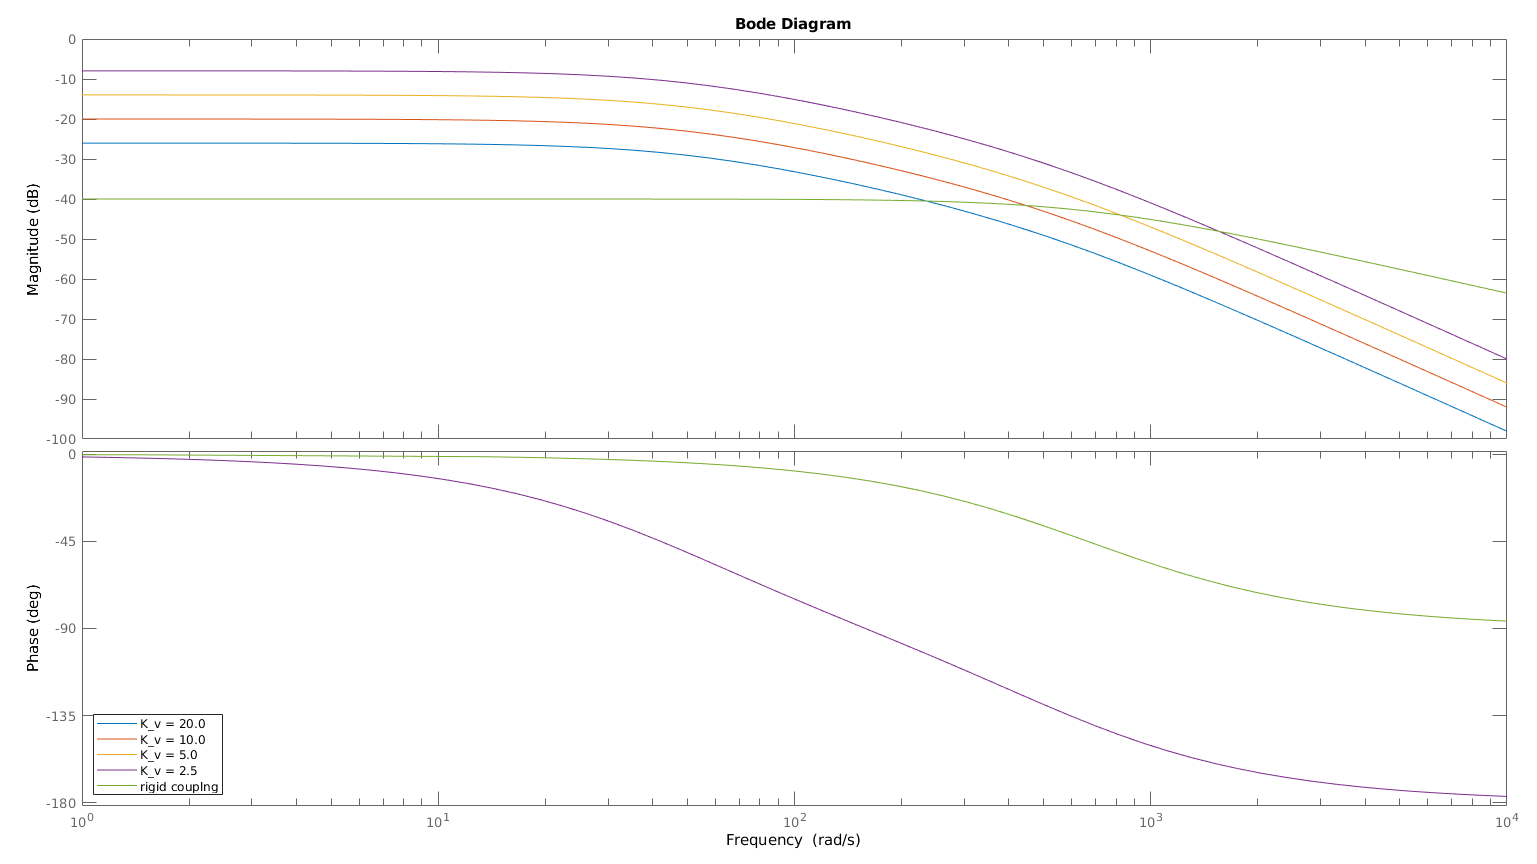
\includegraphics[width=0.7\linewidth]{Images/bodo}
	\caption{Bode diagram of the proposed vibration filter}
	\label{fig:bodo}
\end{figure}

For this reason, in order to reach better task execution performances we want to
reduce the impact of environment vibrations at minimum.
\newline
This could be accomplished, as shown before, by building an ad-hoc filter, such
as fig.\ref{fig:bodo} depicits, in which there are different slope profiles that
will end up rejecting the disturbances at higher frequencies than the
\textsl{cut-off} ones and preserving the signal at lower ones.
\newline
The simulations aims to compare two opposite behaviours: \textbf{rigid coupling}
and \textbf{induced virtual compliance} which is achieved through the choice of
the desired cut-off frequencies.
\newline

In particular these frequencies correspond respectively to 8 and 80 Htz.
It is interesting the comparison of the vibration suppression applied on three
different noise frequencies:

\begin{itemize}
\item $10^{1} Htz$ : In fig.\ref{fig:10Htz} is shown how the vibrations at lower frequencies are preserved by the
\textsl{virtual compliance}, this is a rather enticing aspect of a teleoperation interaction
since the input commands generated by the controller will have kind of low frequencies.
\item $10^{2} Htz$ : The fig.\ref{fig:100Htz} demonstrates a turning point in which the
disturbance rejection achieved by the \textsl{rigid coupling} is comparable to
the performance of \textsl{virtual compliance}.
\item $10^{3} Htz$ At frequencies higher than the cut-off ones, the
vibrations will be dumped more effectively by the sets of computed virtual
parameters than with \textsl{rigid coupling}, this is deducible from fig.\ref{fig:1000Htz}.
\end{itemize}

\begin{figure}[h]
	\begin{subfigure}[h!]{1\linewidth}
		\centering
		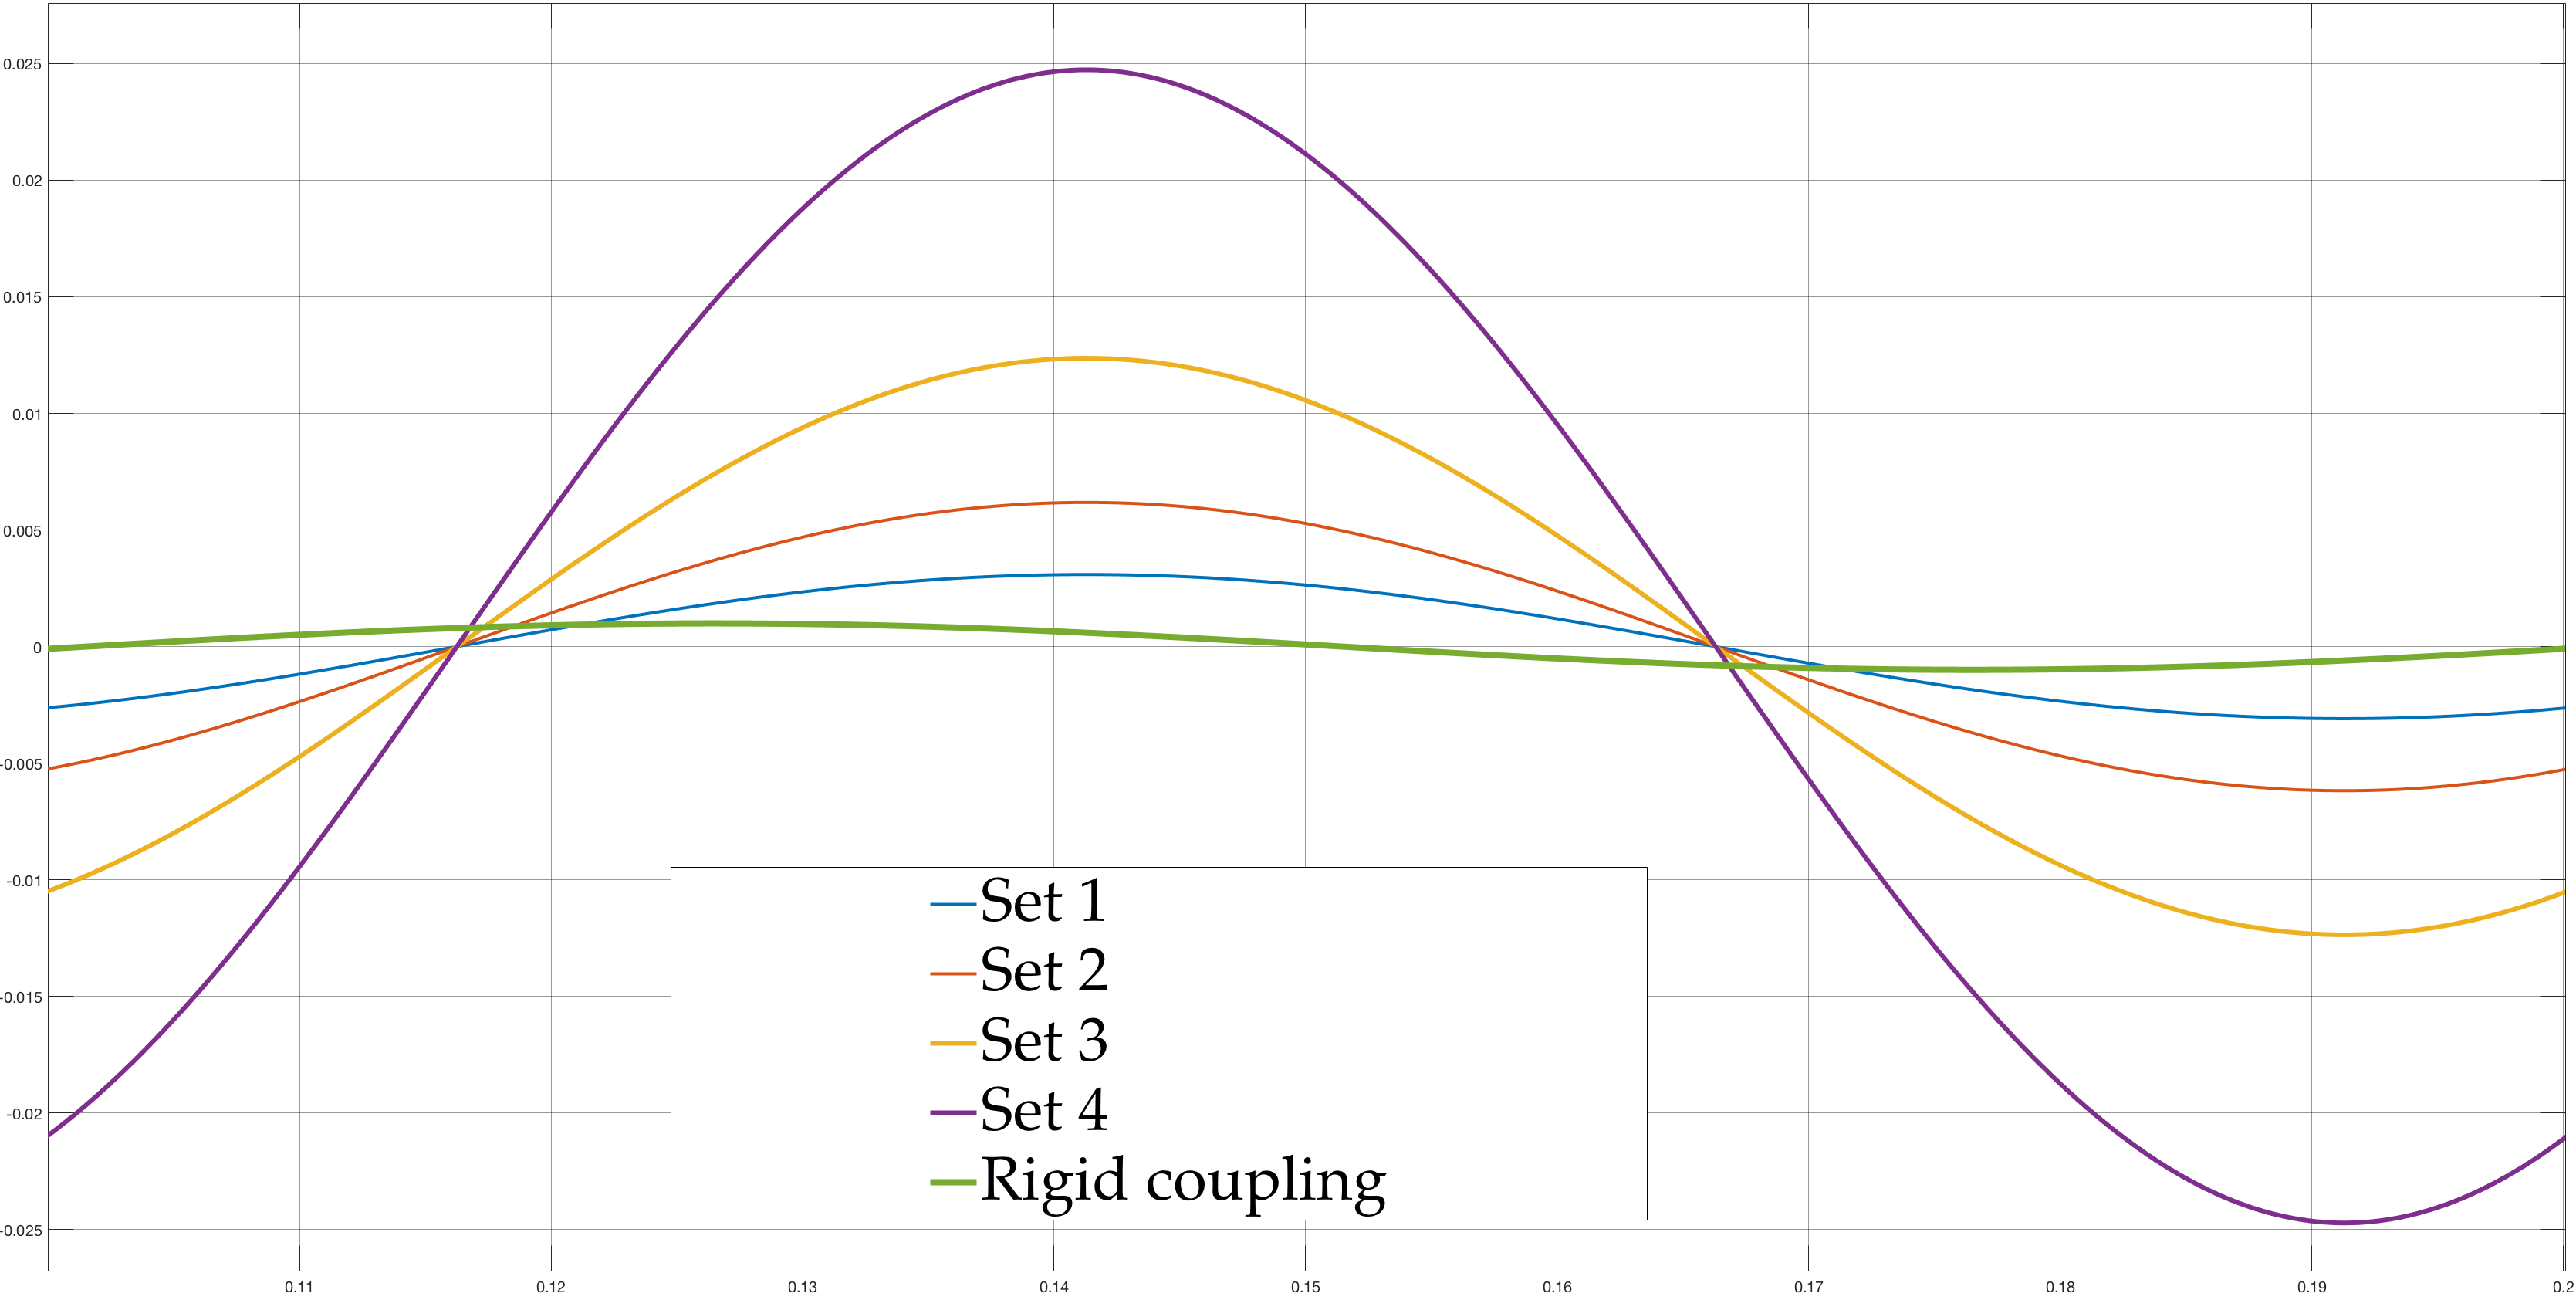
\includegraphics[width=\textwidth, height=0.29\textwidth]{Images/vibr10Htz}
		\caption{10 Htz}
		\label{fig:10Htz}
	\end{subfigure}	
  \newline
	\begin{subfigure}[h!]{1\linewidth}
		\centering
		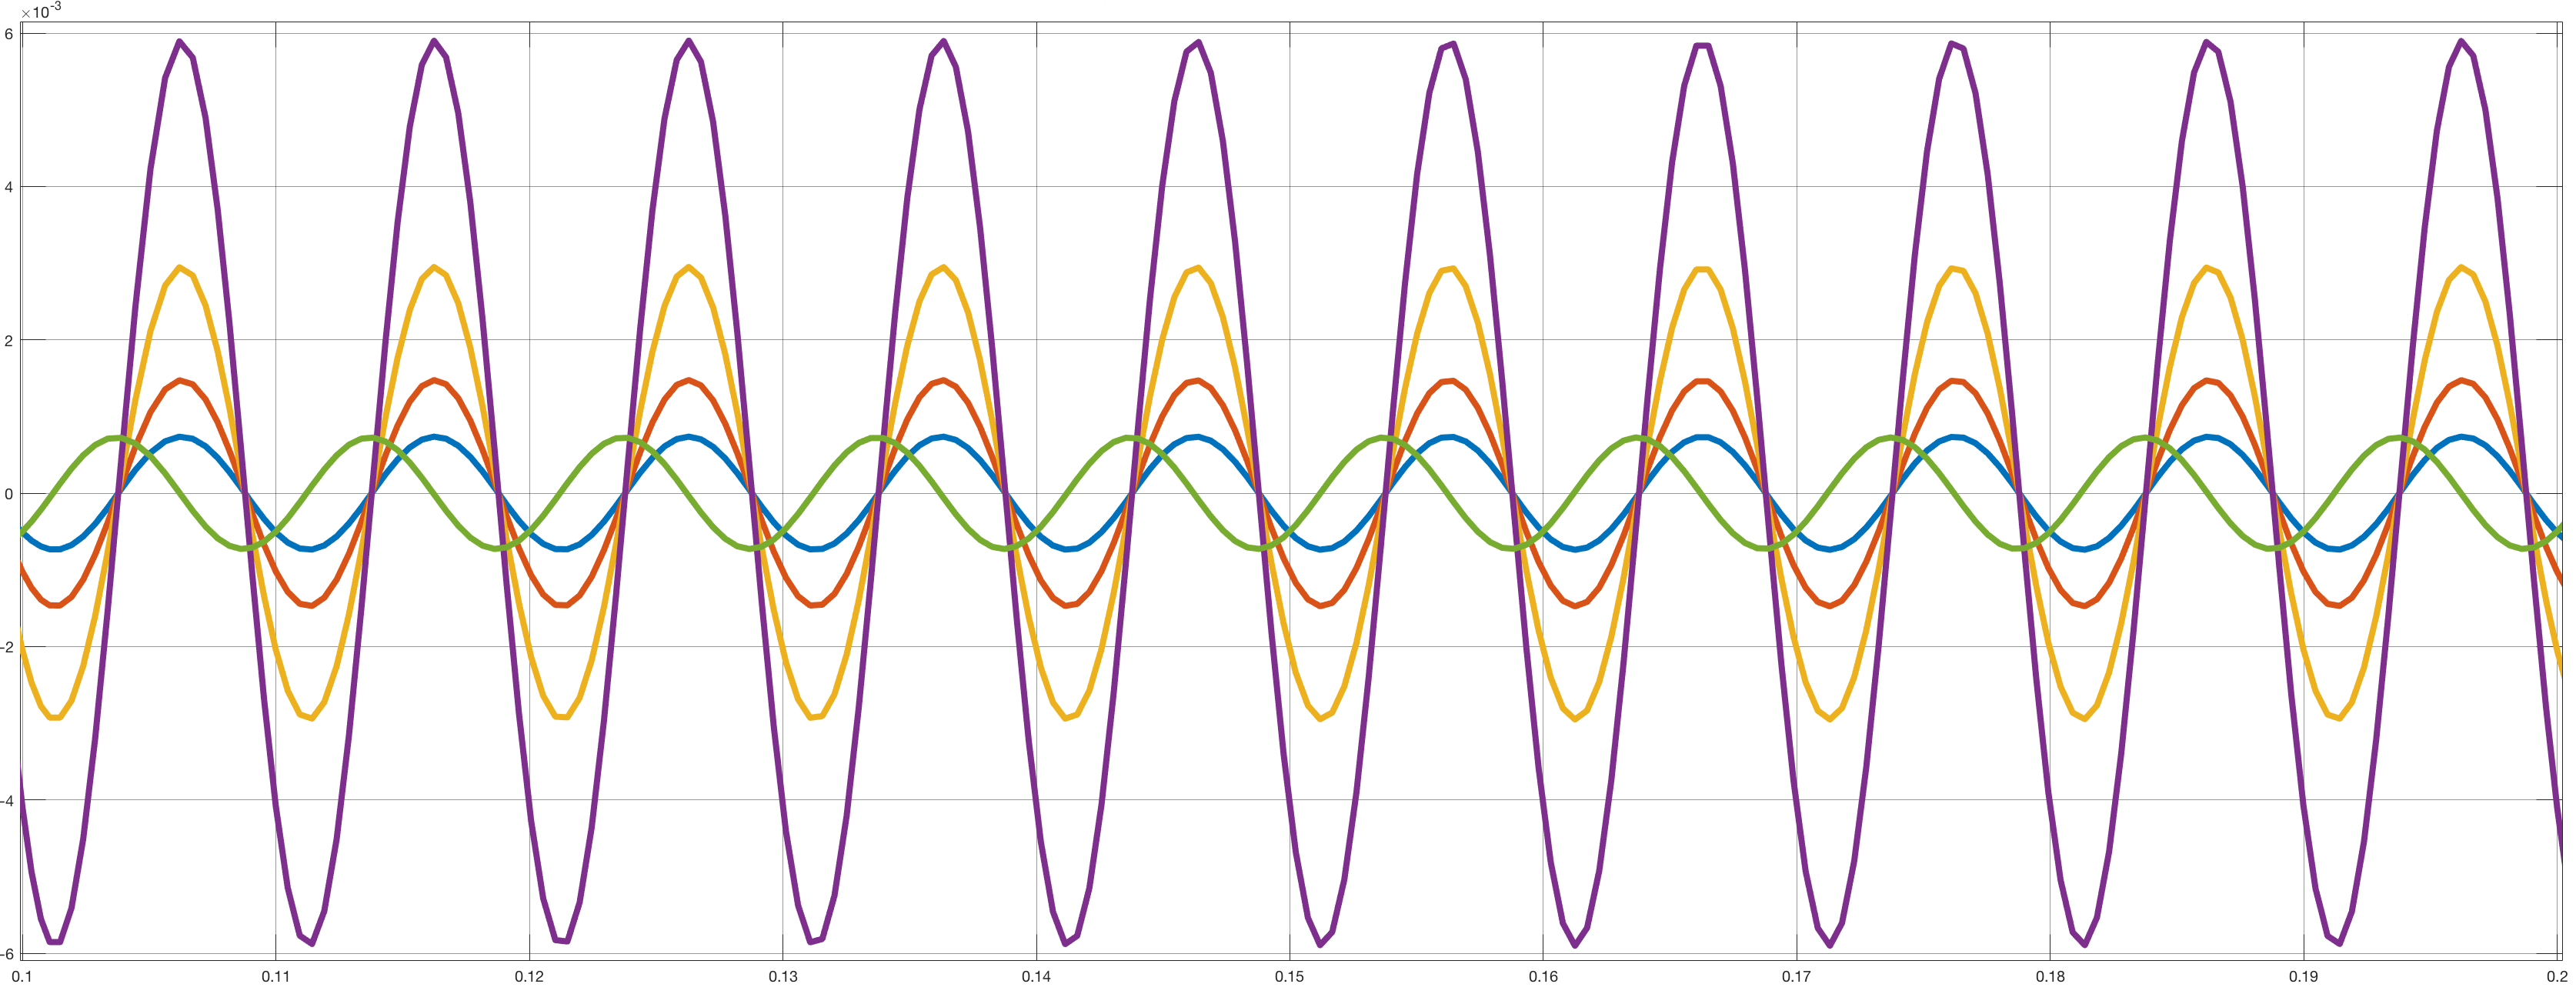
\includegraphics[width=\textwidth, height=0.29\textwidth]{Images/vibr100Htz}
		\caption{100 Htz}
		\label{fig:100Htz}
	\end{subfigure}	
  \newline
	\begin{subfigure}[h!]{1\linewidth}
		\centering.
		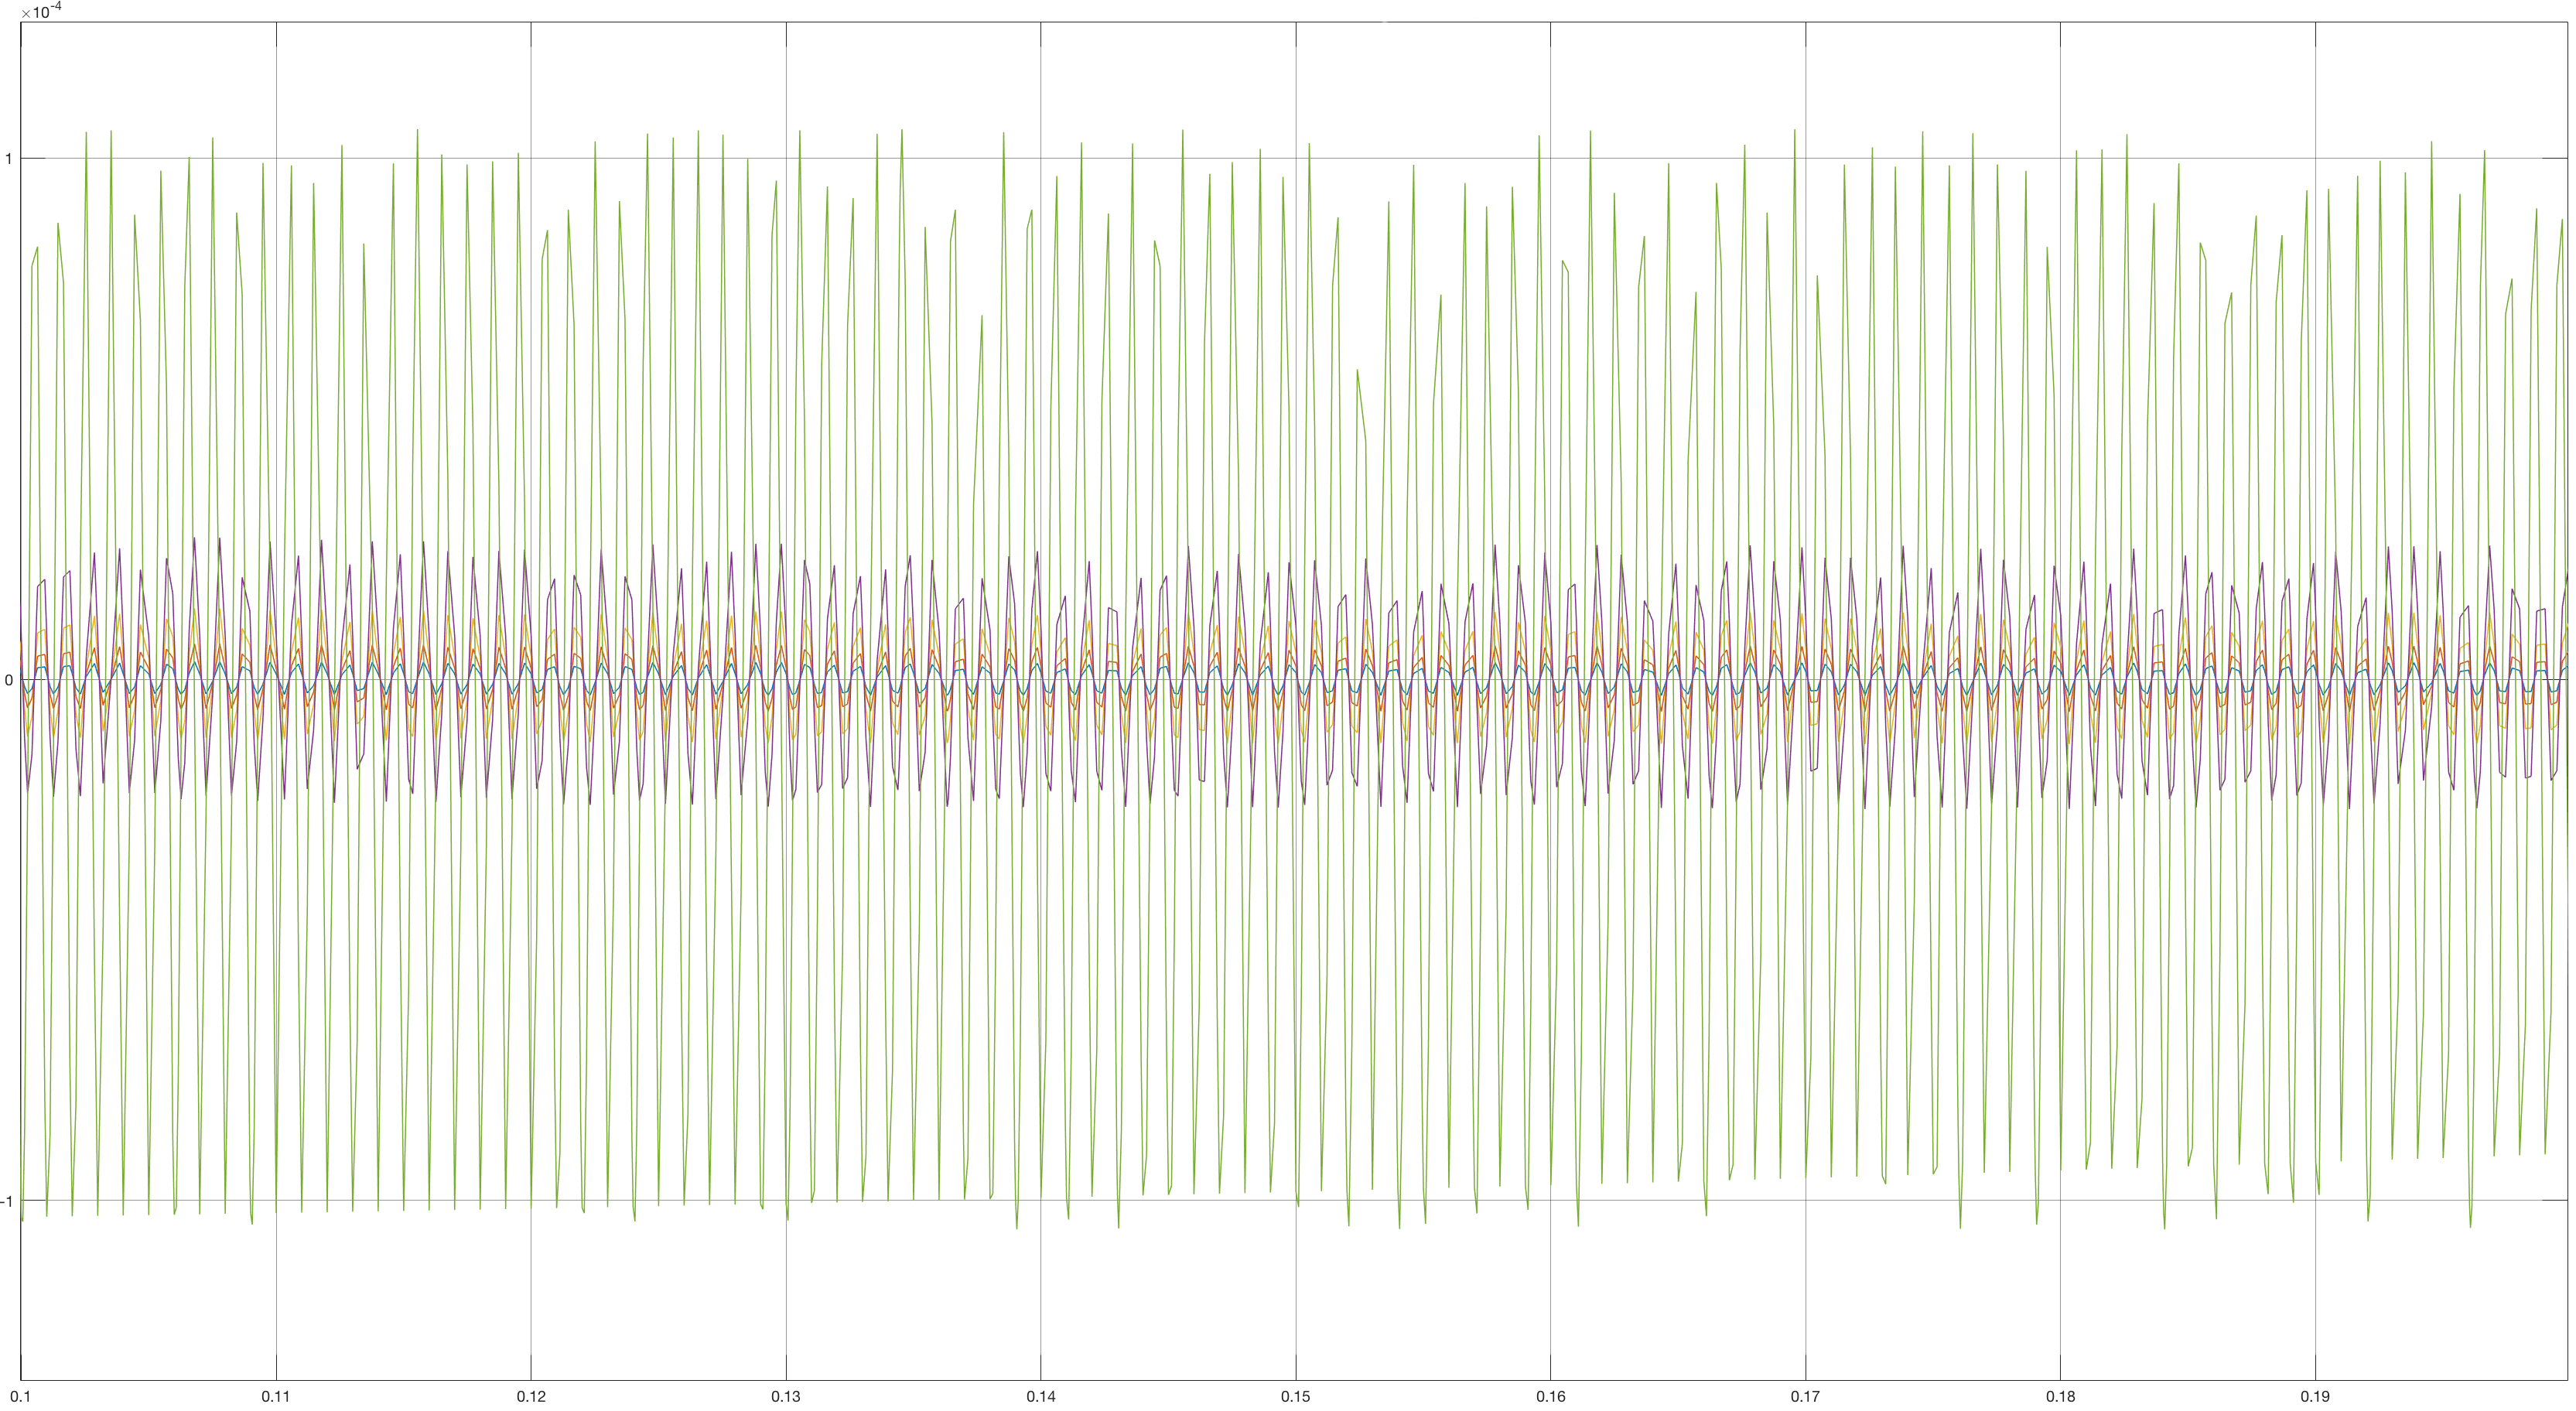
\includegraphics[width=\textwidth, height=0.29\textwidth]{Images/vibr1000Htz}
		\caption{1000 Htz}
		\label{fig:1000Htz}
	\end{subfigure}
\caption{ Signal response to a noise with three different frequencies modulated 
  by the proposed vibration damping filter.}
\end{figure}

\newpage

\subsection{Task execution analysis}

\subsubsection{Free motion with high noise frequencies}

At first, we present an execution in free motion where , the
slave manages to mirror the master which moves according to a sinusoidal
trajectory,
applying both \textsl{rigid coupling} (fig.\ref{fig:freeRigTot50HR}) and
\textsl{virtual compliance} (fig.\ref{fig:freeSetTot50HR}), with almost no task error
(without considering the error due to noise disturbances).


\begin{figure}[h]
	\begin{subfigure}[h!]{1\linewidth}
		\centering
		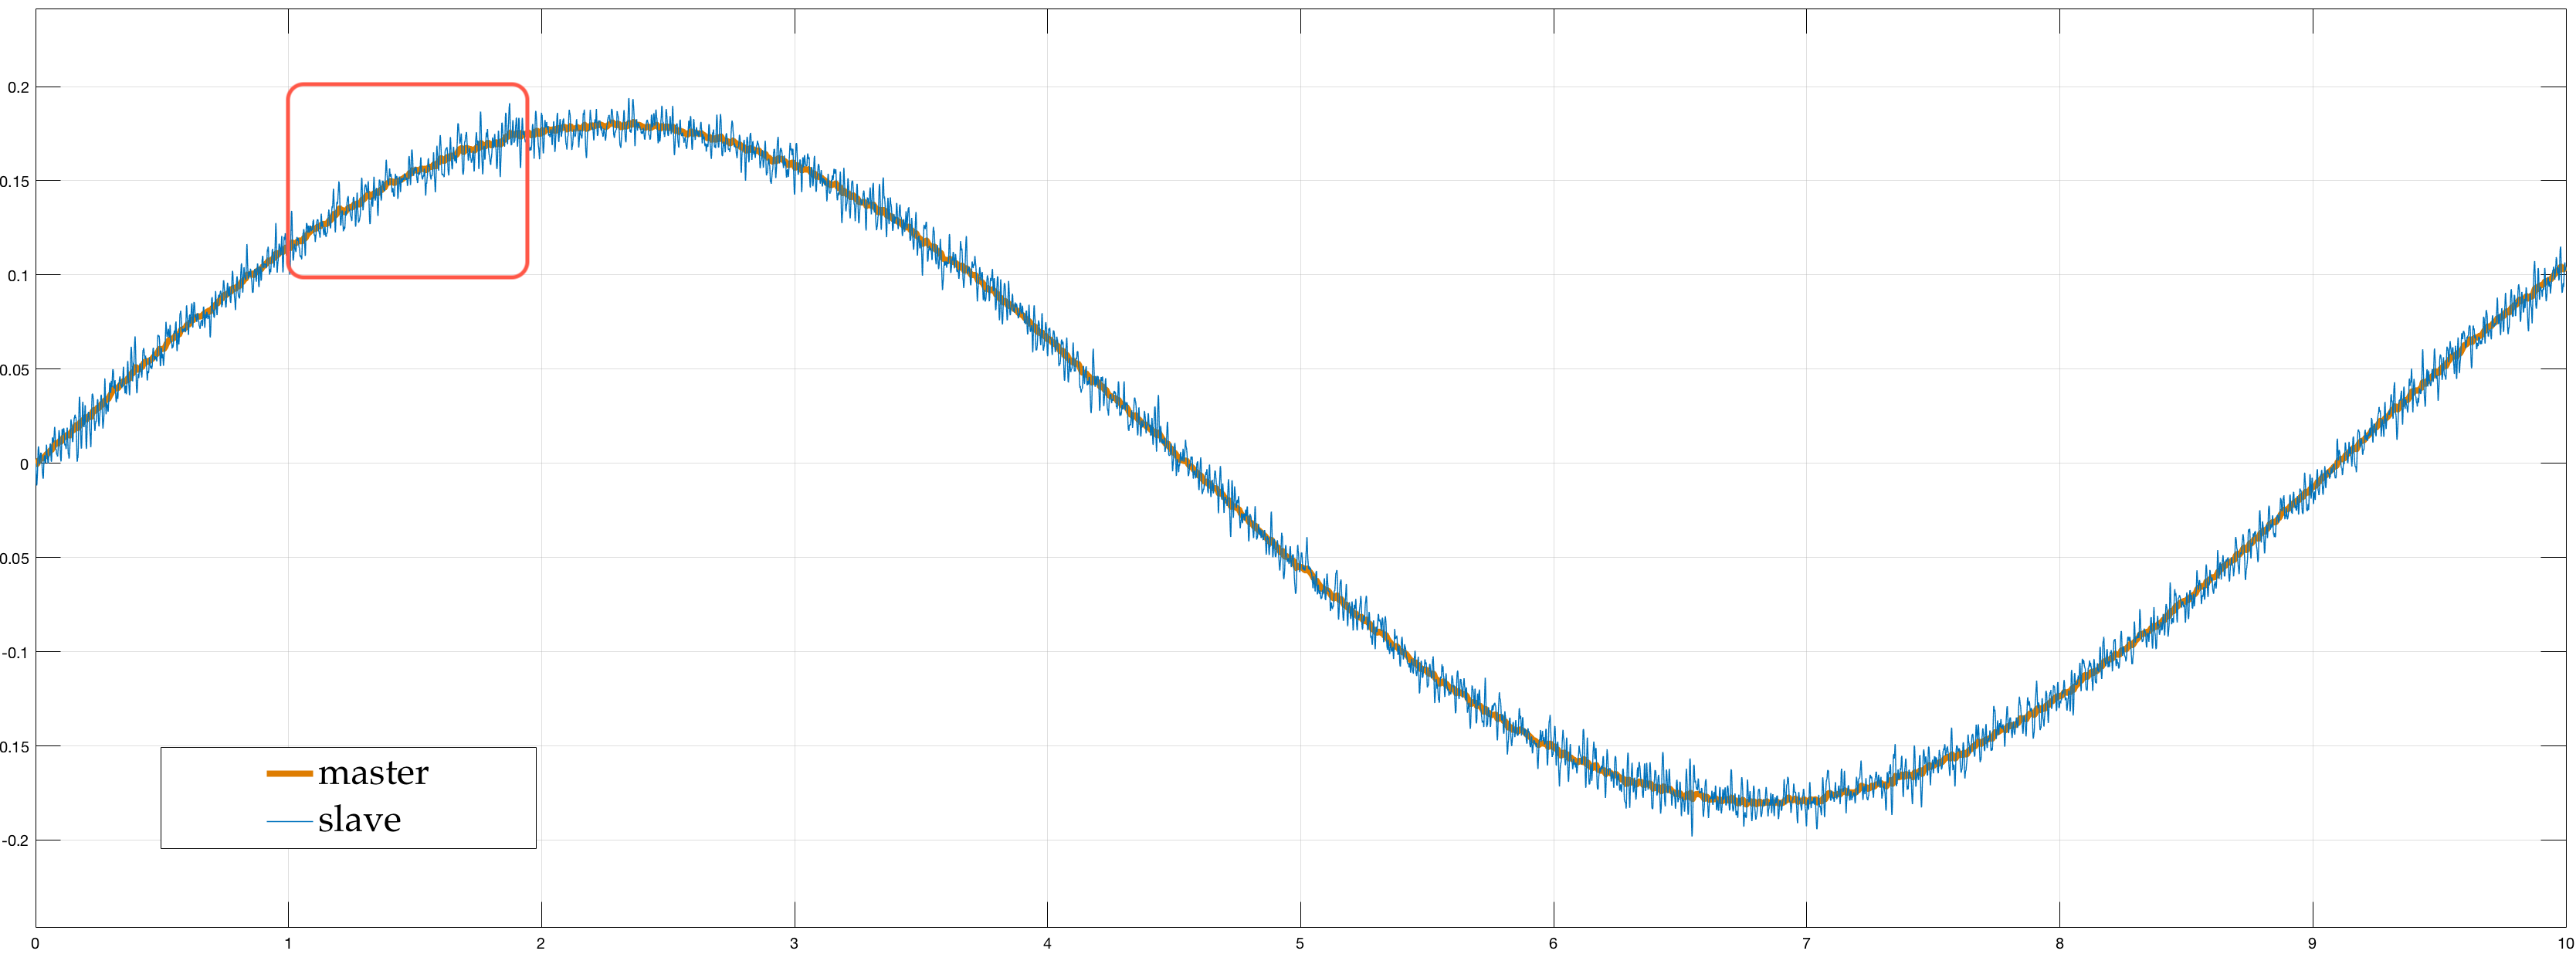
\includegraphics[width=\textwidth, height=0.48\textwidth]{Images/rCoupFreeTot50htznoiseRect}
		\caption{Angular positions assumed during trajectory tracking}
		\label{fig:freeRigTot50HR}
	\end{subfigure}	
  \newline
	\begin{subfigure}[h!]{1\linewidth}
		\centering
		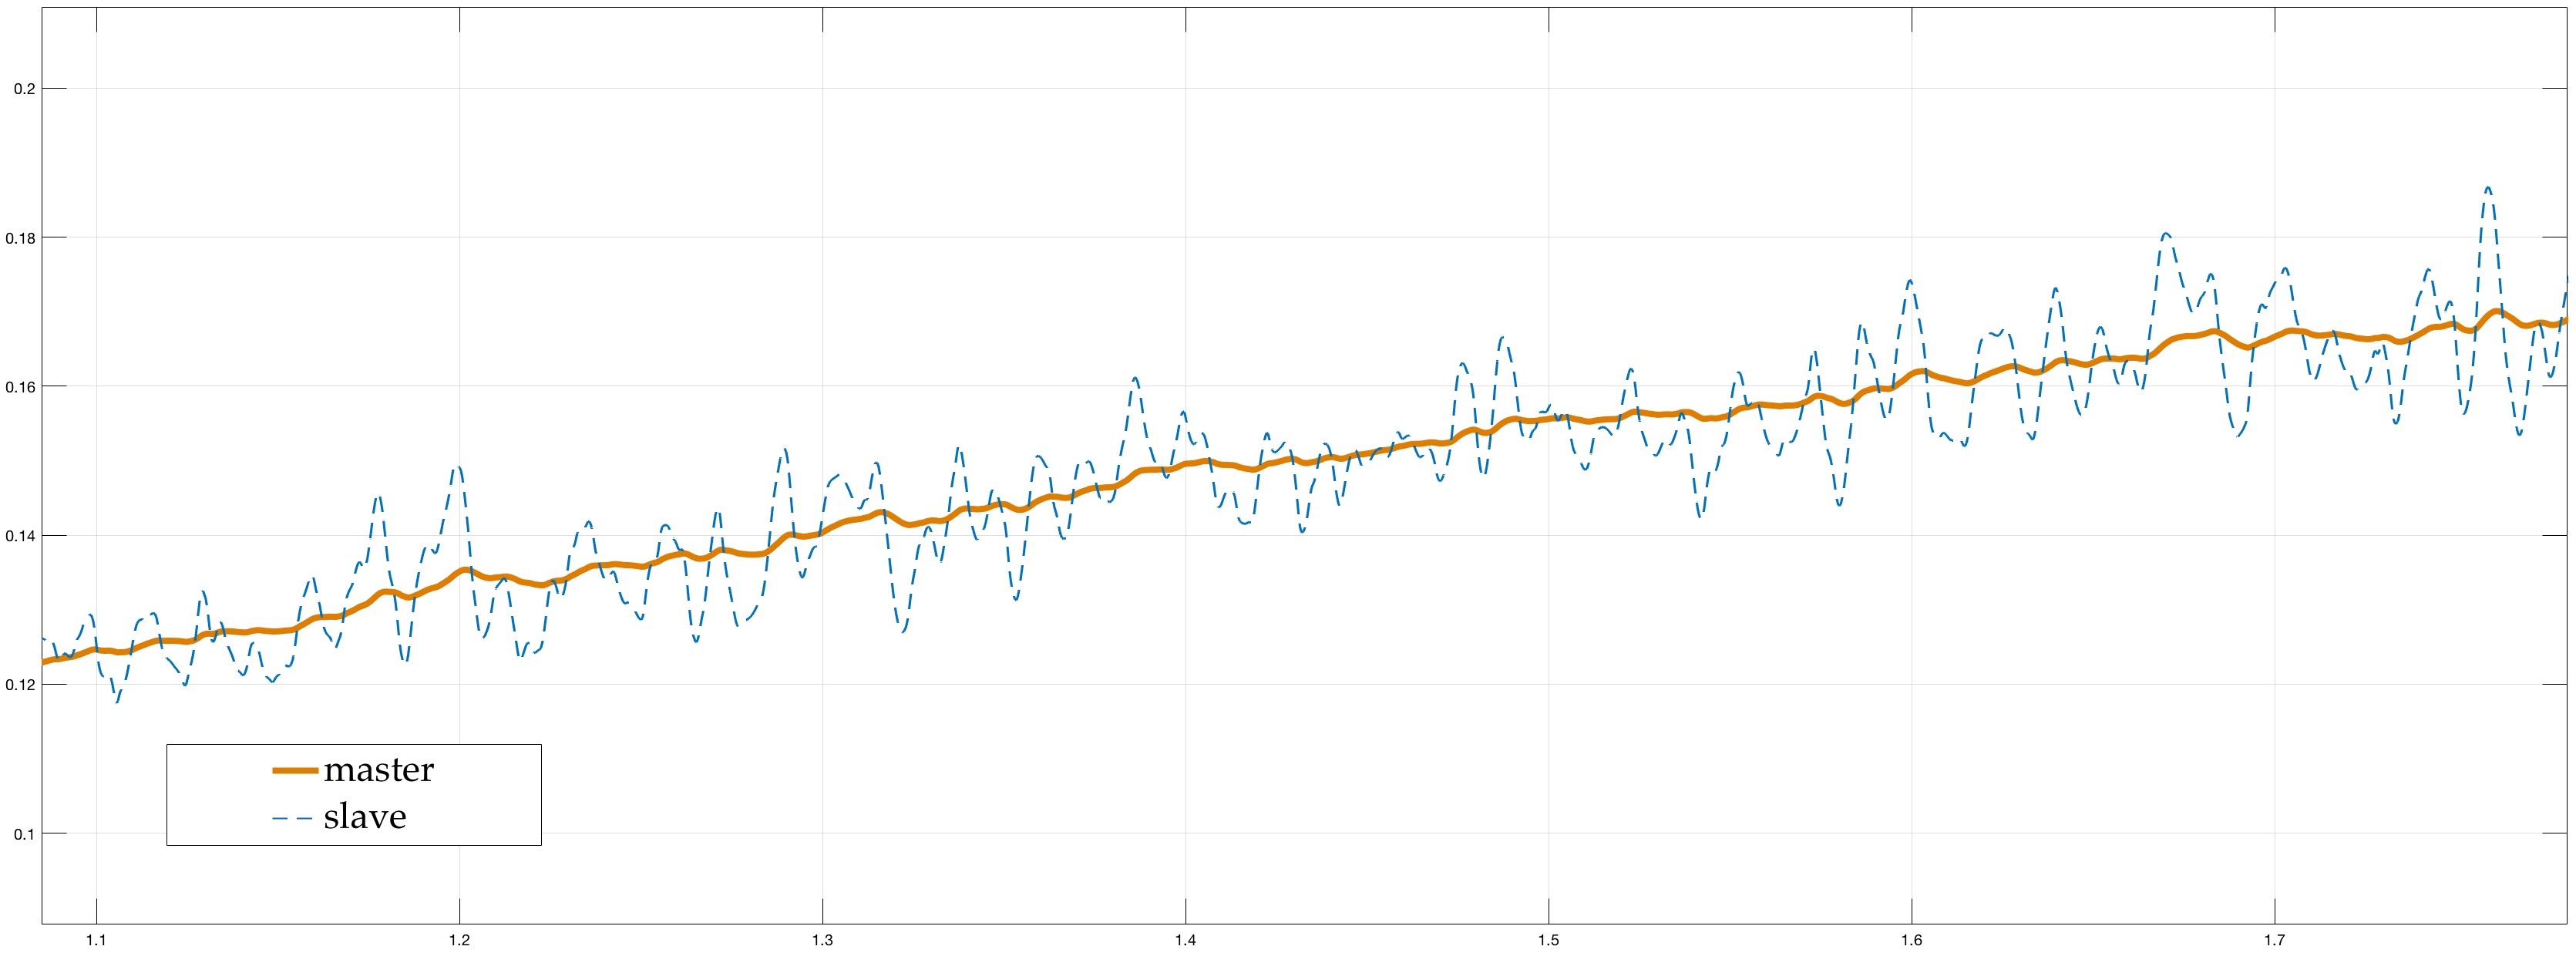
\includegraphics[width=\textwidth, height=0.48\textwidth]{Images/rCoupFree50htznoise}
		\caption{Detail describing the highlighted area in fig.\ref{fig:freeRigTot50HR}}
		\label{fig:freeRigPar50HR}
	\end{subfigure}	
  \caption{ Rigid coupling simulation under \textbf{high} frequency disturbances. }
\end{figure}

\newpage

Actually, the noise of the system has been built through a mixture of white
noise and sinusoidal oscillations both at frequency of $5\cdot 10^{1} Htz$.
\newline
This kind of disturbance should be damped, and in fact, using \textsl{virtual
  compliance} (fig.\ref{fig:freeRigPar50HR}) the profile of the angle is smoother
than in \textsl{rigid coupling} (fig.\ref{fig:freeSetPar50HR}).

\bigskip


\begin{figure}[h]
	\begin{subfigure}[h!]{1\linewidth}
		\centering
		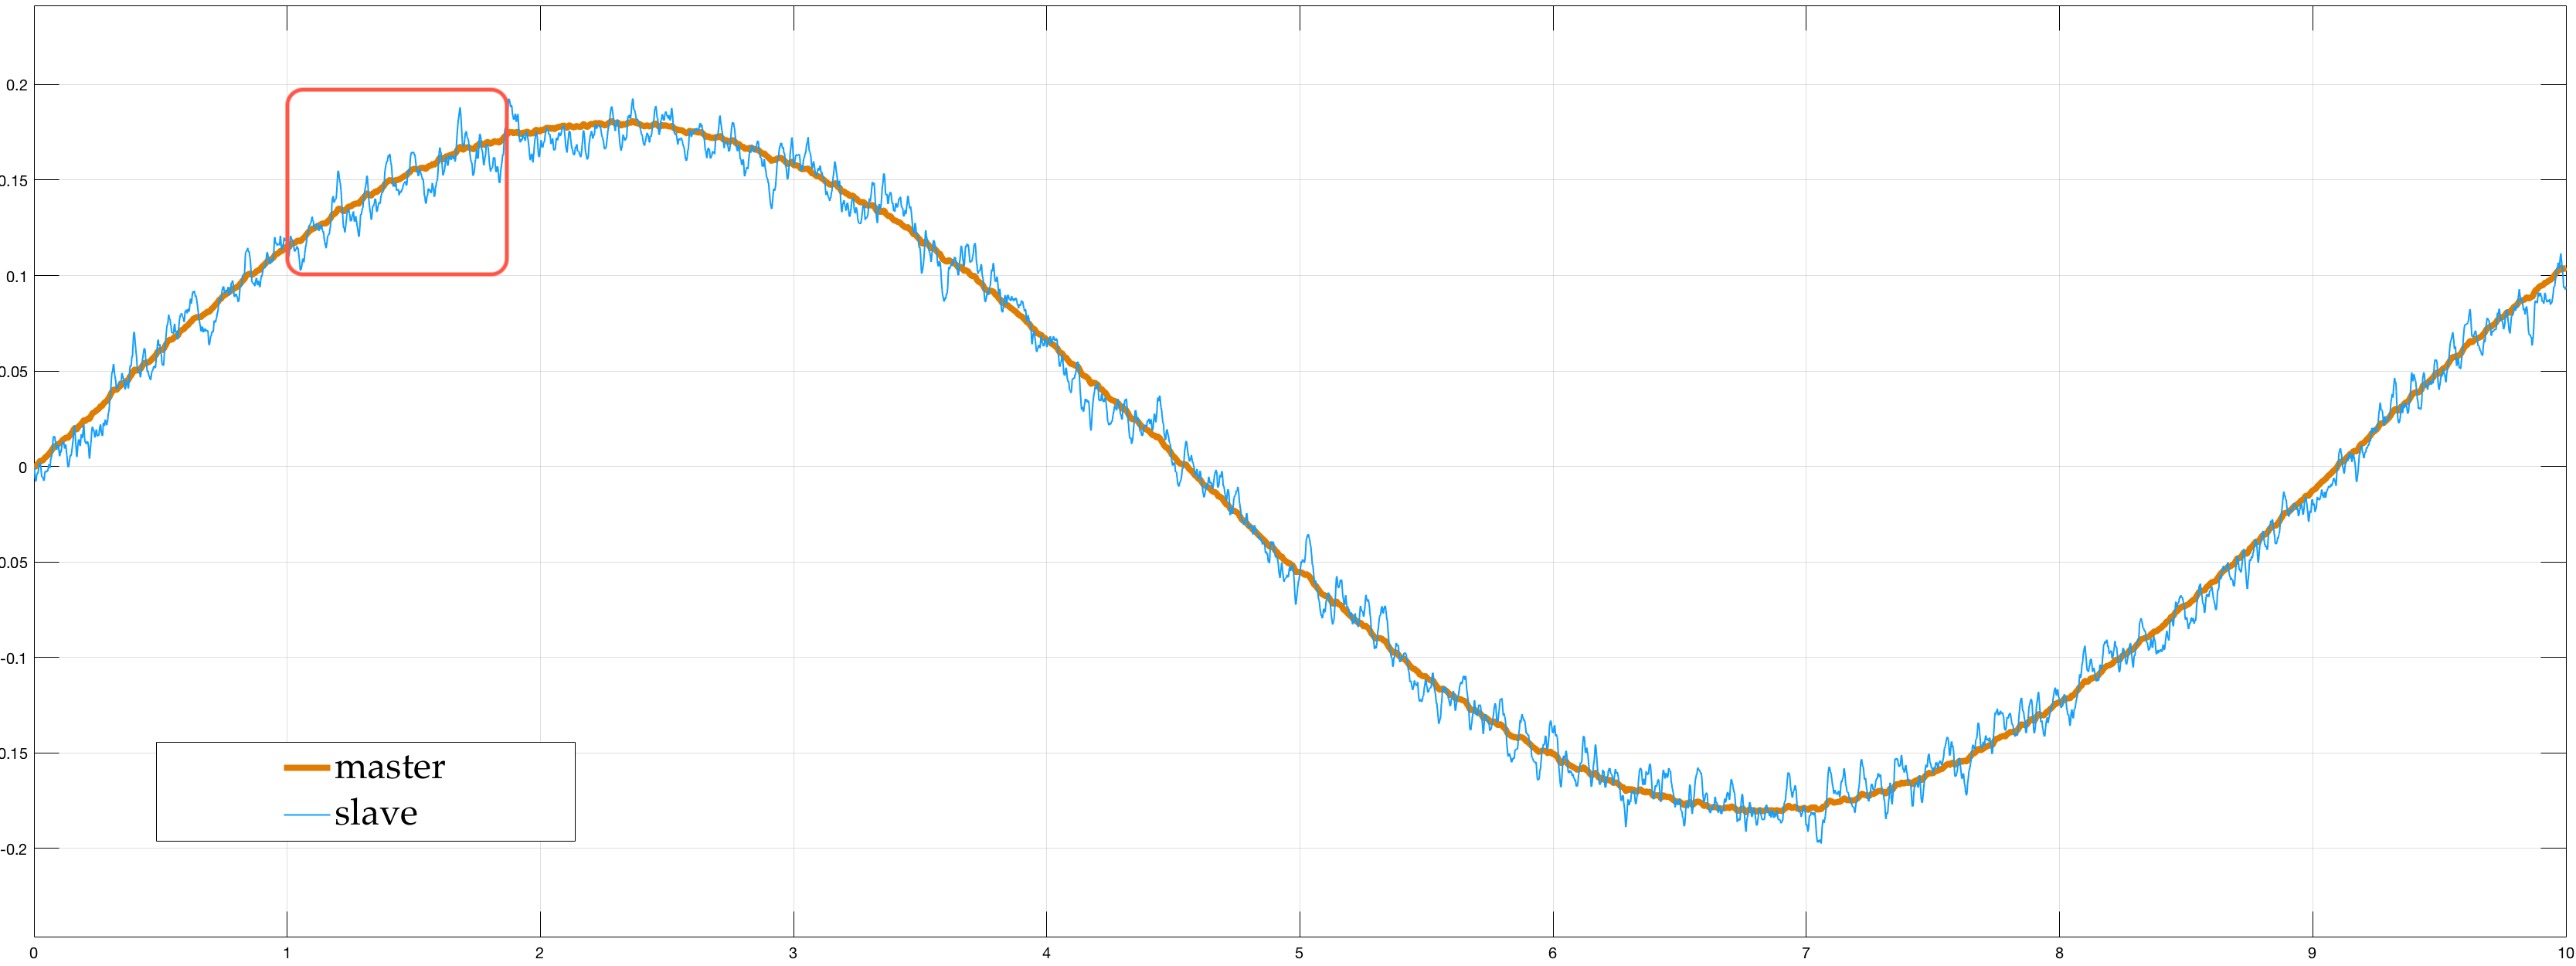
\includegraphics[width=\textwidth, height=0.48\textwidth]{Images/set20freeTot50HtznoiseRect}
		\caption{Angular positions assumed during trajectory tracking}
		\label{fig:freeSetTot50HR}
	\end{subfigure}	
  \newline
	\begin{subfigure}[h!]{1\linewidth}
		\centering
		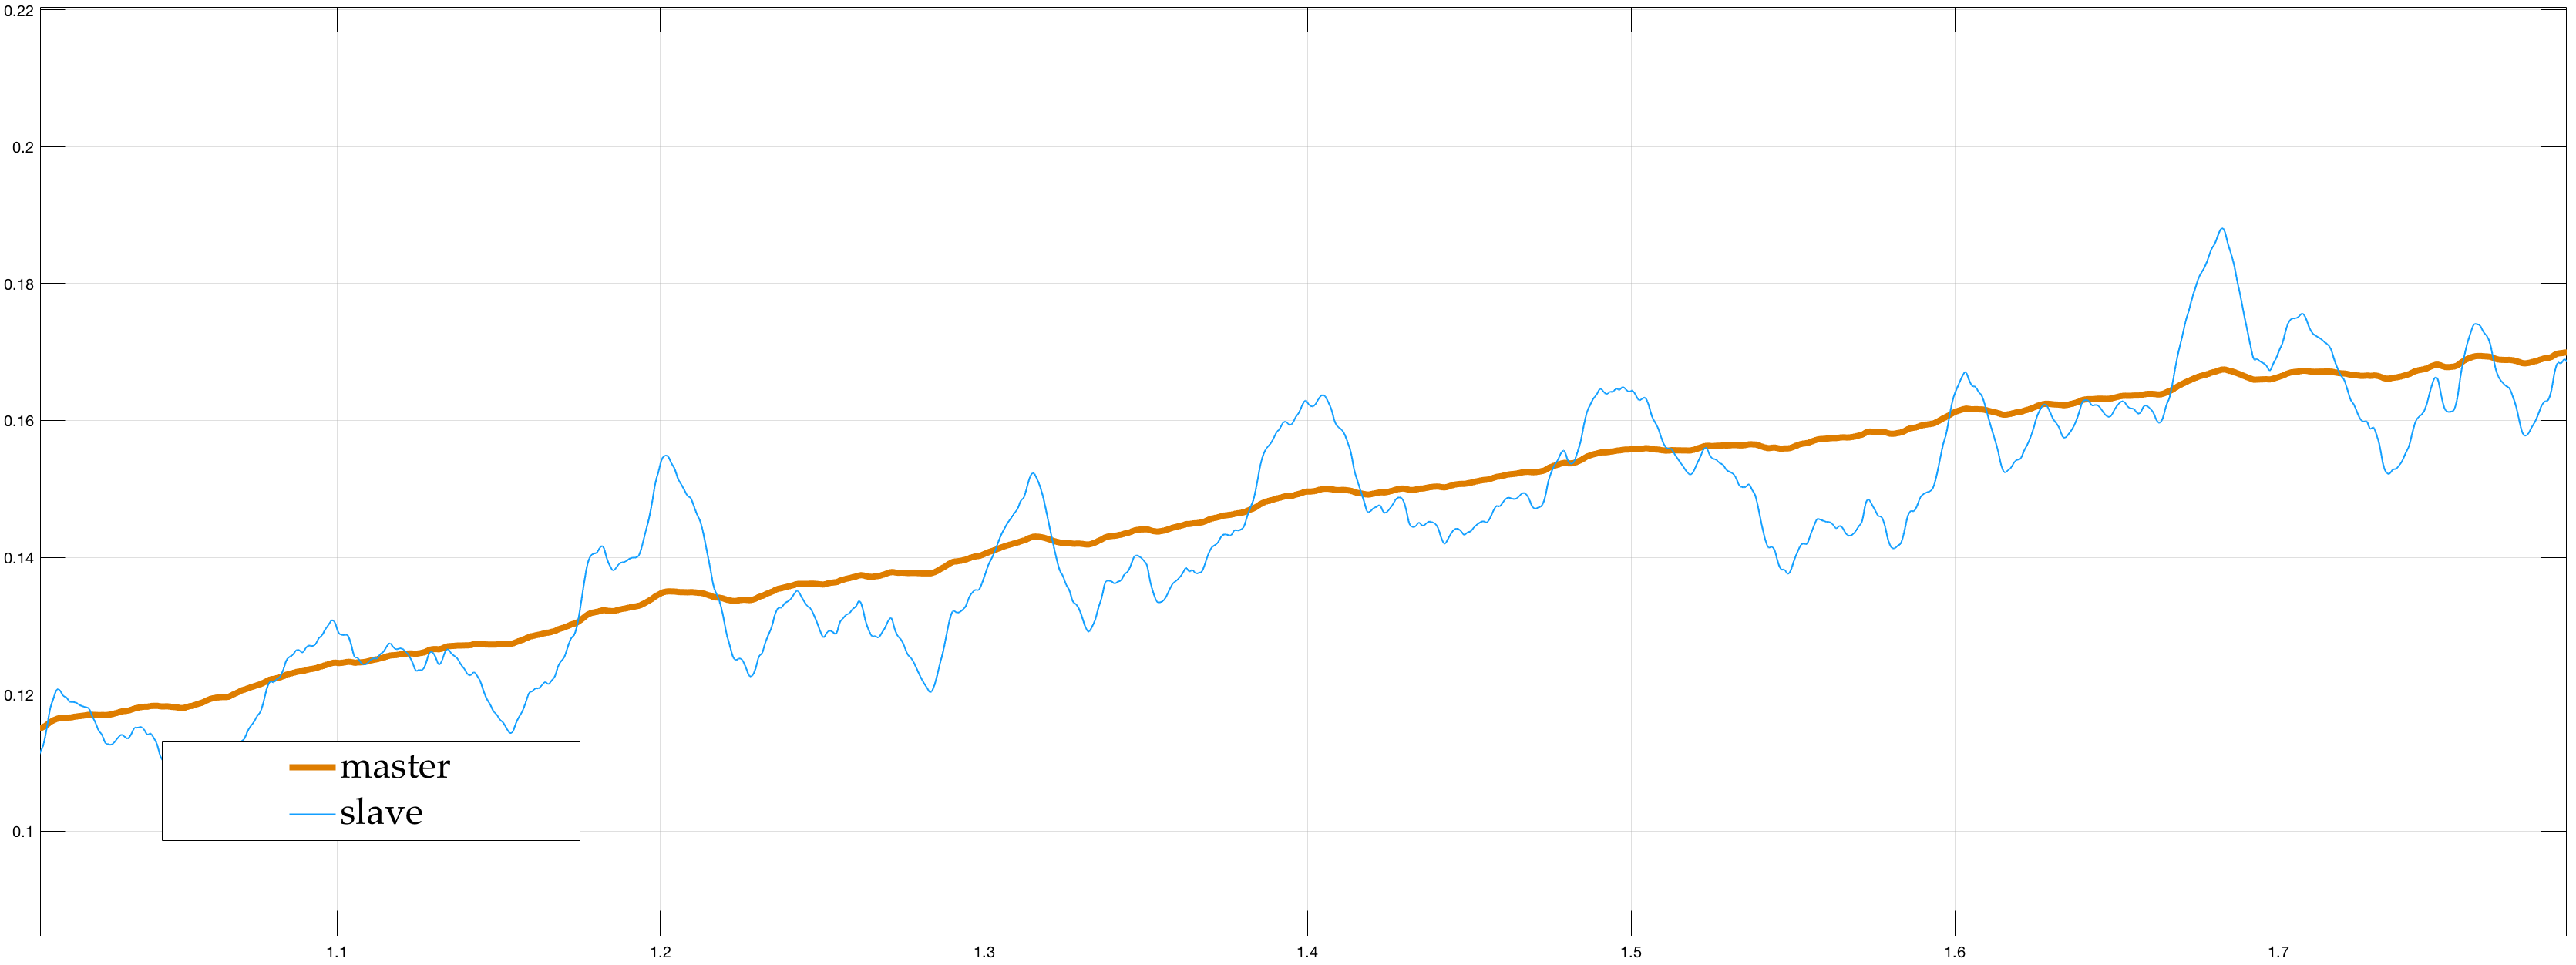
\includegraphics[width=\textwidth, height=0.48\textwidth]{Images/set20freePart50Htznoise}
		\caption{Detail describing the highlighted area in fig.\ref{fig:freeSetTot50HR}}
		\label{fig:freeSetPar50HR}
	\end{subfigure}	
  \caption{ Virtual compliance simulation under \textbf{high} frequency disturbances. }
\end{figure}





\newpage
\subsubsection{Free motion with low noise frequencies}

Comparatively, two other simulations have been undertaken that share the same
conditions of the previous ones, if not for the noise frequency, which has been
lowered to $2\cdot 10^{1} Htz$.
\newline
This kind of disturbance is usually a similar to the input of the control
actuators, so it should be preserved, namely it shouldn't be affected by the
proposed filtering.

\begin{figure}[h]
	\begin{subfigure}[h!]{1\linewidth}
		\centering
		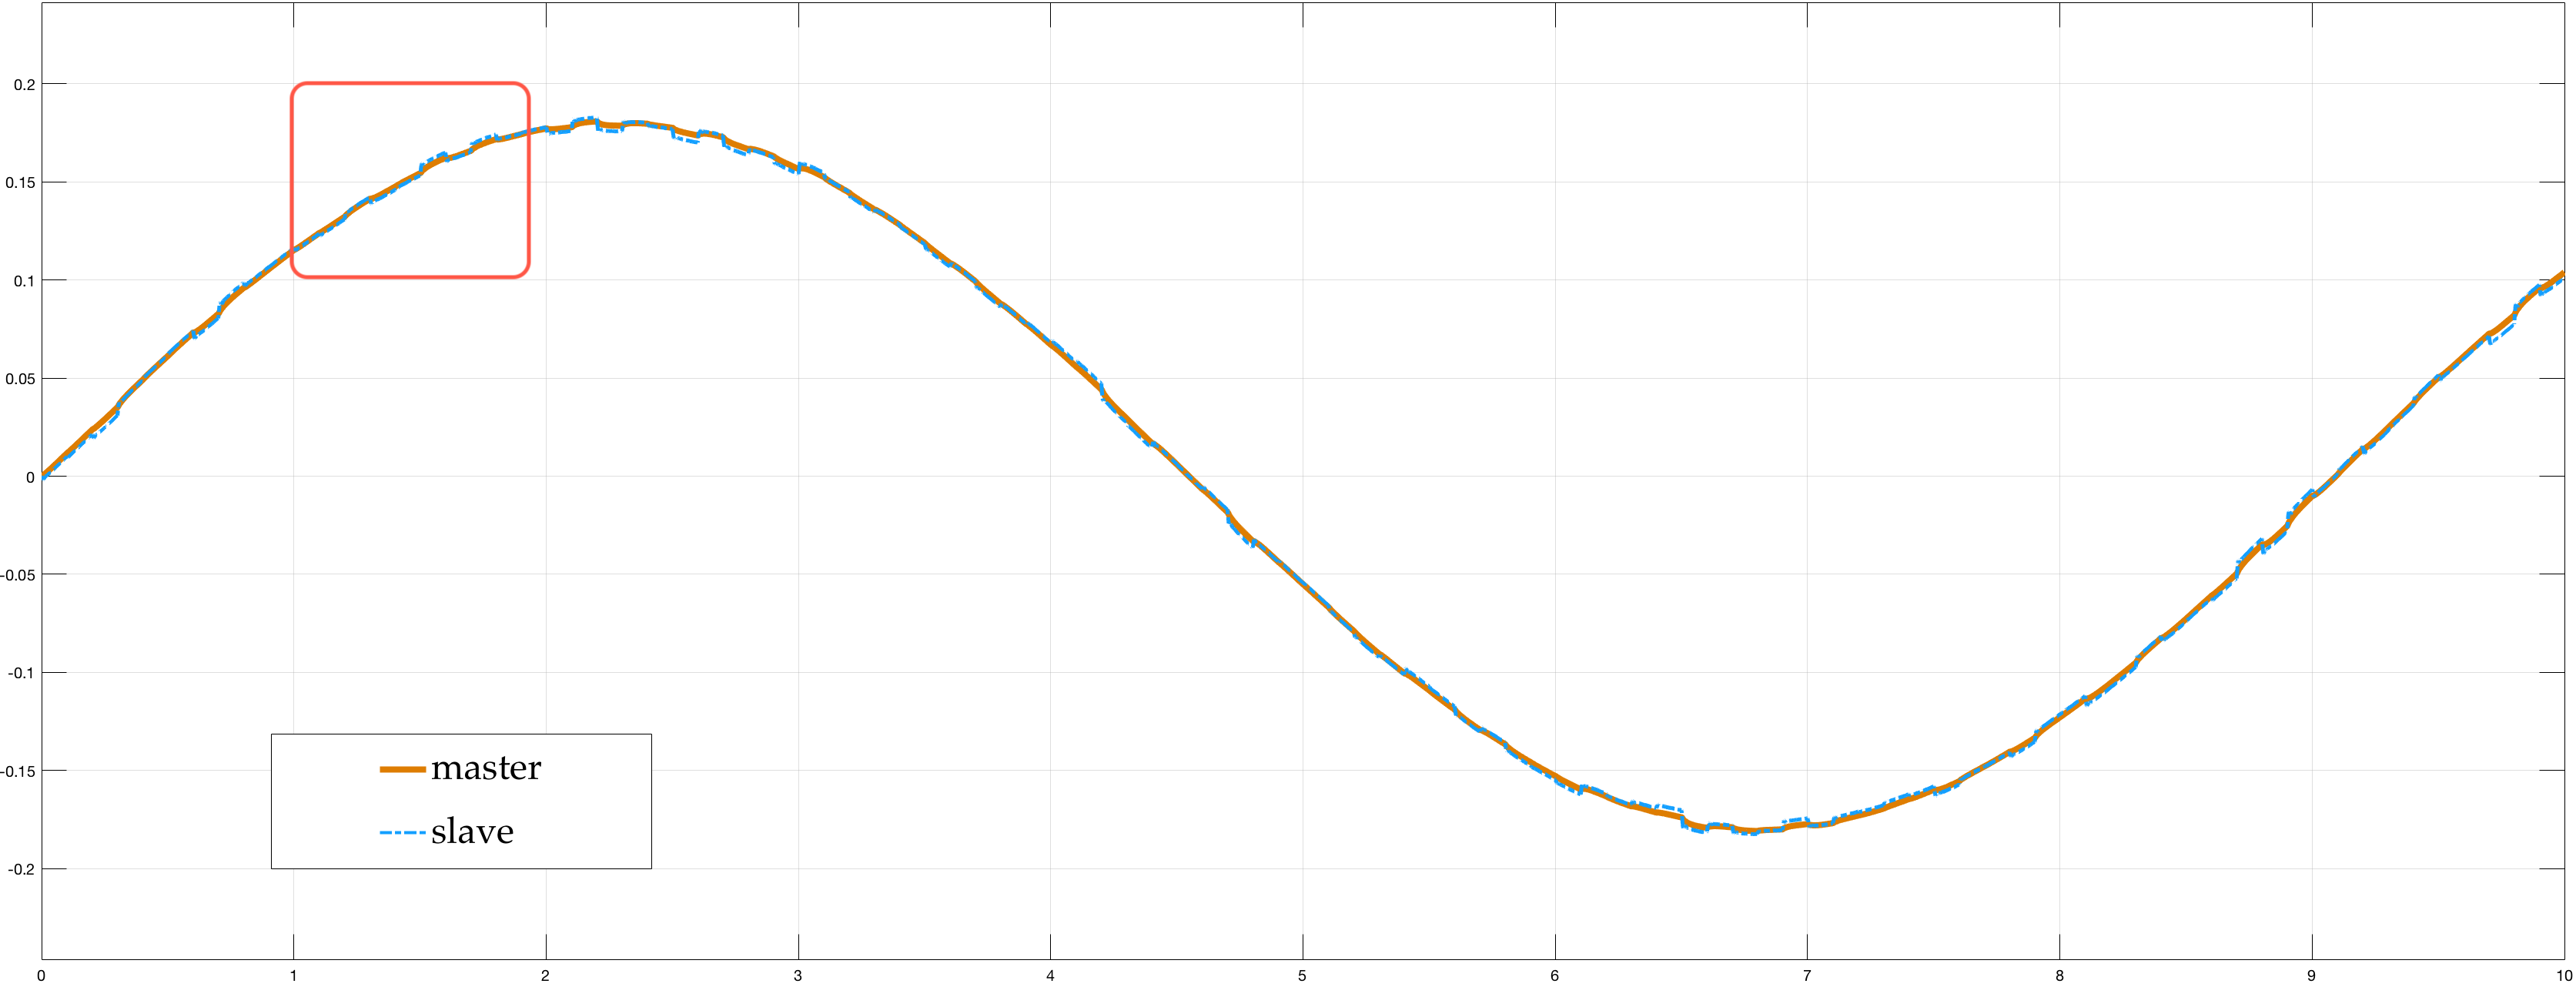
\includegraphics[width=\textwidth, height=0.48\textwidth]{Images/freerigidTot20HtznoiseRect}
		\caption{Angular positions angles assumed during trajectory tracking.}
		\label{fig:freeRigTot20HR}
	\end{subfigure}	
  \newline
	\begin{subfigure}[h!]{1\linewidth}
		\centering
		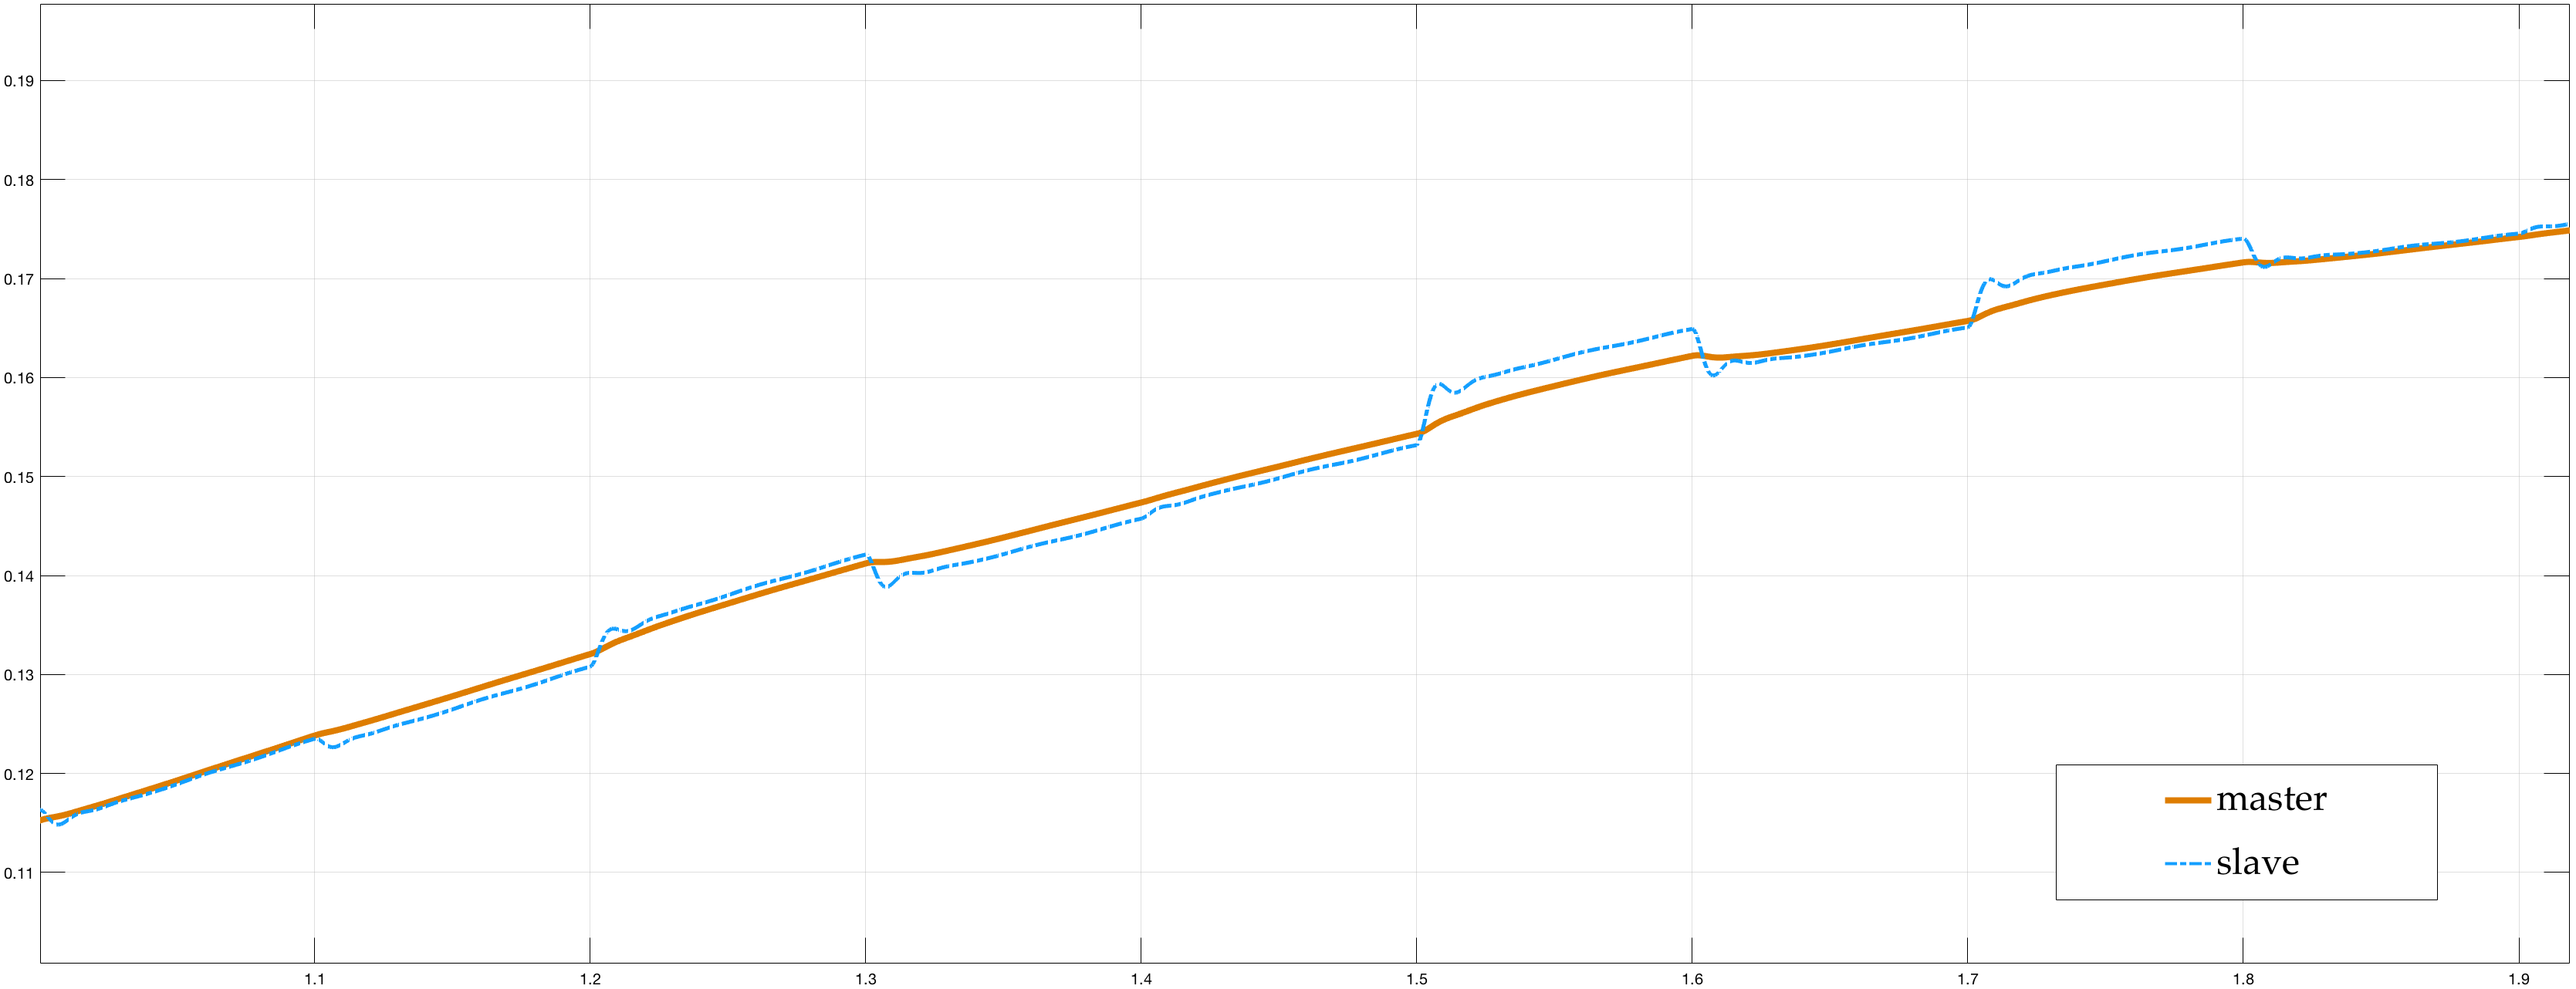
\includegraphics[width=\textwidth, height=0.48\textwidth]{Images/freerigidPart20Htznoise}
		\caption{Detail describing the highlighted area in fig.\ref{fig:freeRigTot20HR}}
		\label{fig:freeRigPar20HR}
	\end{subfigure}	
 \caption{ Rigid coupling simulation under \textbf{low} frequency disturbances.}
\end{figure}


This phenomenon shows up in fig.\ref{fig:freeRigPar20HR} and fig.\ref{fig:freeSetPar20HR}.
In fact, if compared, the two profiles confirm that \textsl{rigid coupling}
cancel out most of the useful information from the signal.
\newline
On the contrary \textsl{virtual compliance} save the signal information,
which is extremely important from a control perspective.



  
\begin{figure}[h]
	\begin{subfigure}[h!]{1\linewidth}
		\centering
		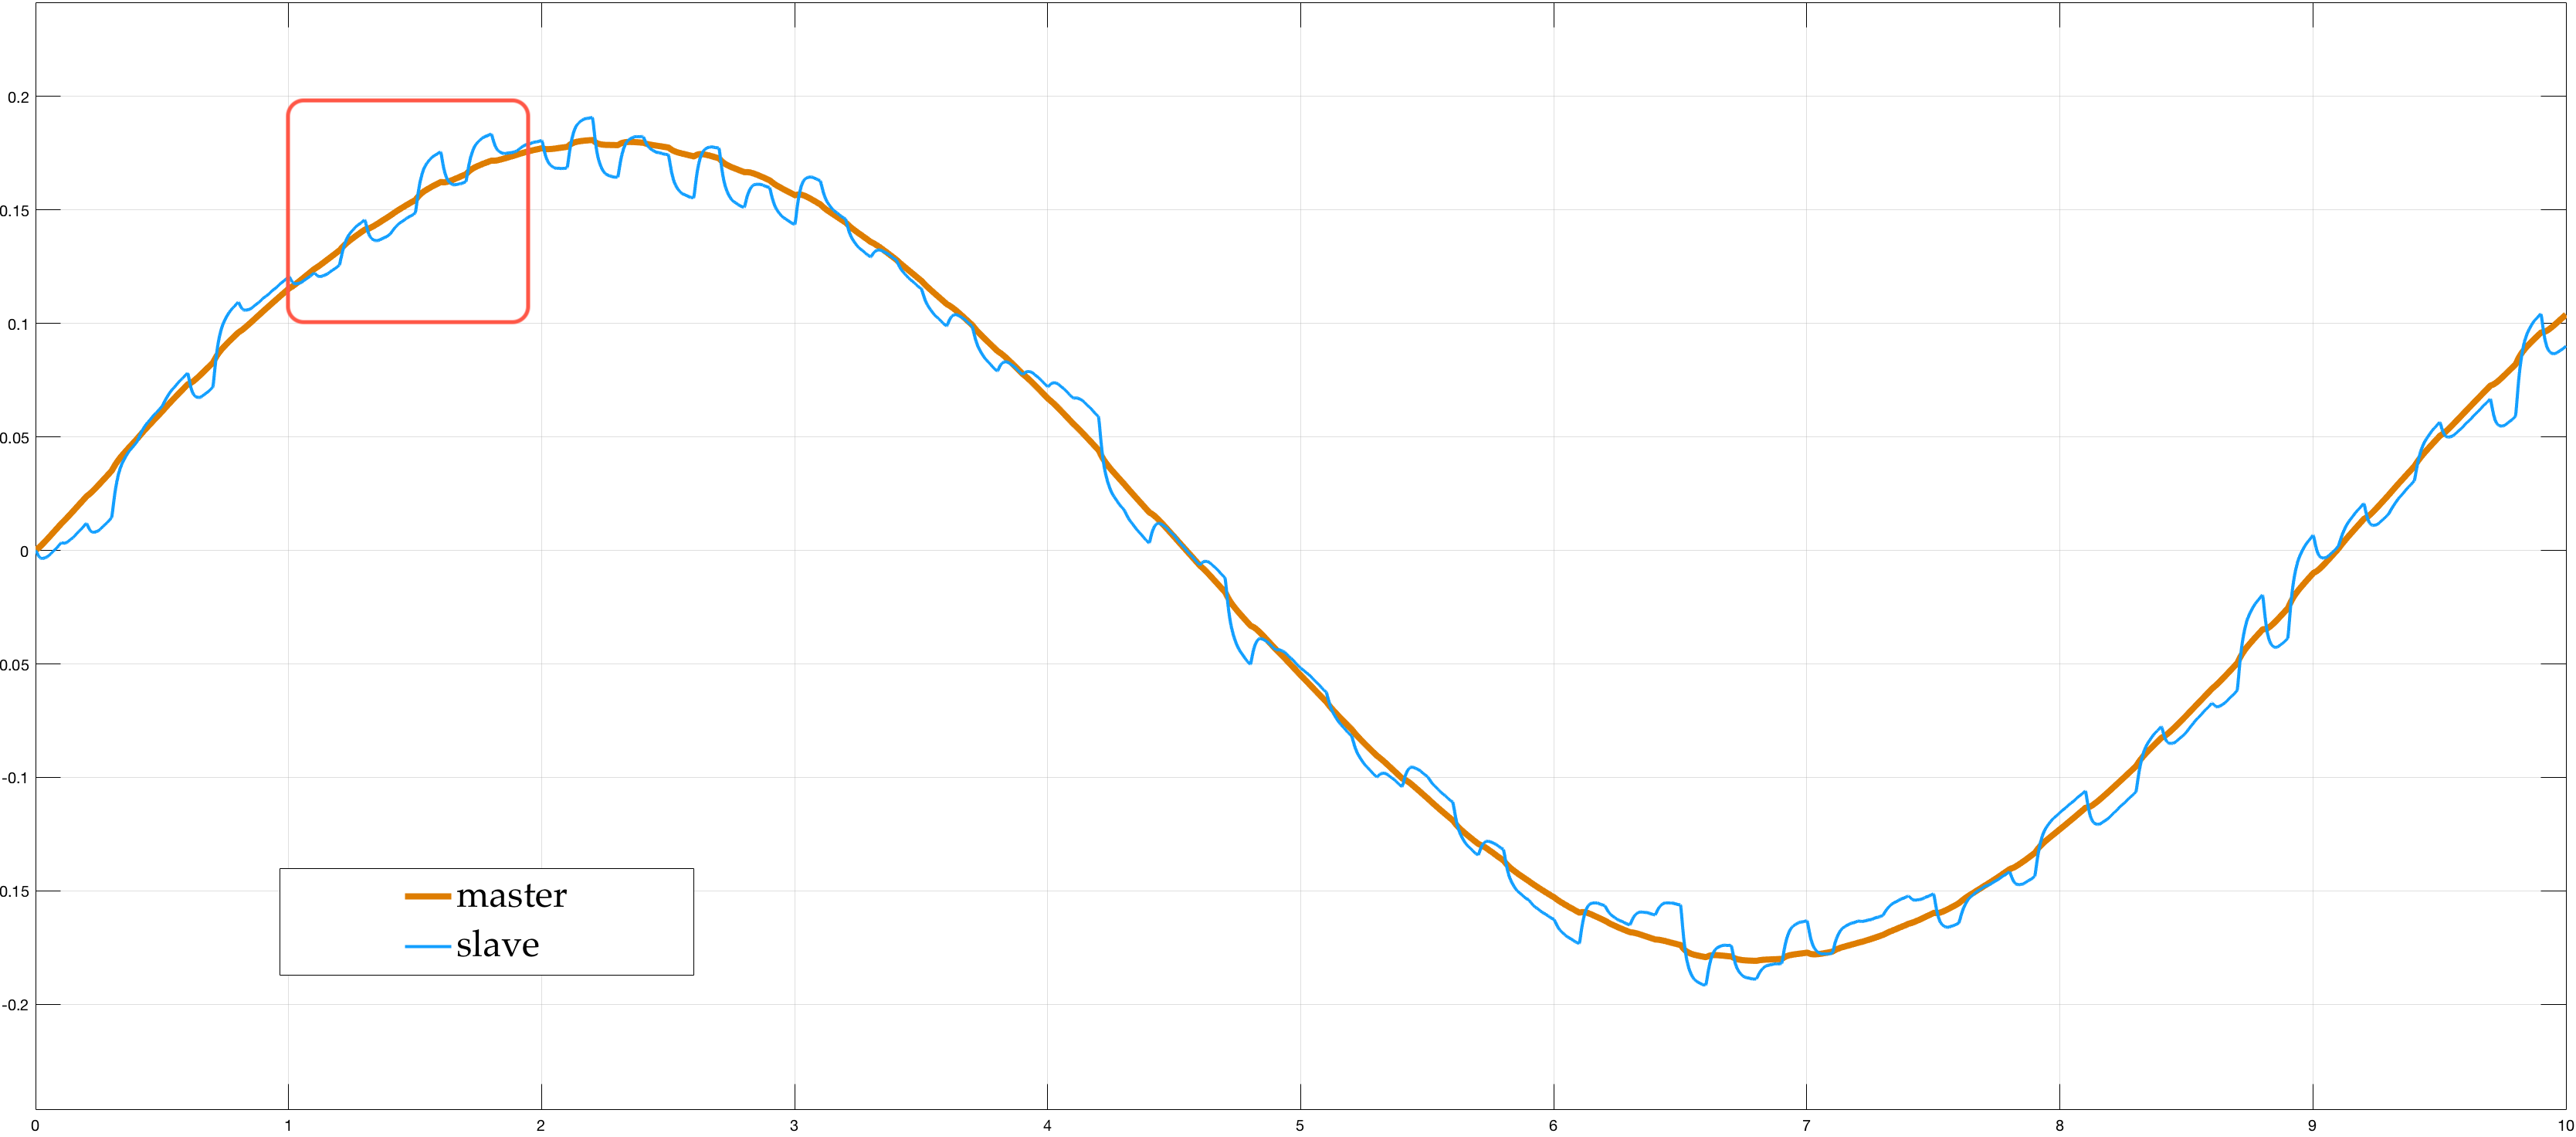
\includegraphics[width=\textwidth, height=0.48\textwidth]{Images/freeSet20Tot20HtznoiseRect}
		\caption{Angular position assumed during trajectory tracking.}
		\label{fig:freeSetTot20HR}
	\end{subfigure}	
  \newline
	\begin{subfigure}[h!]{1\linewidth}
		\centering
		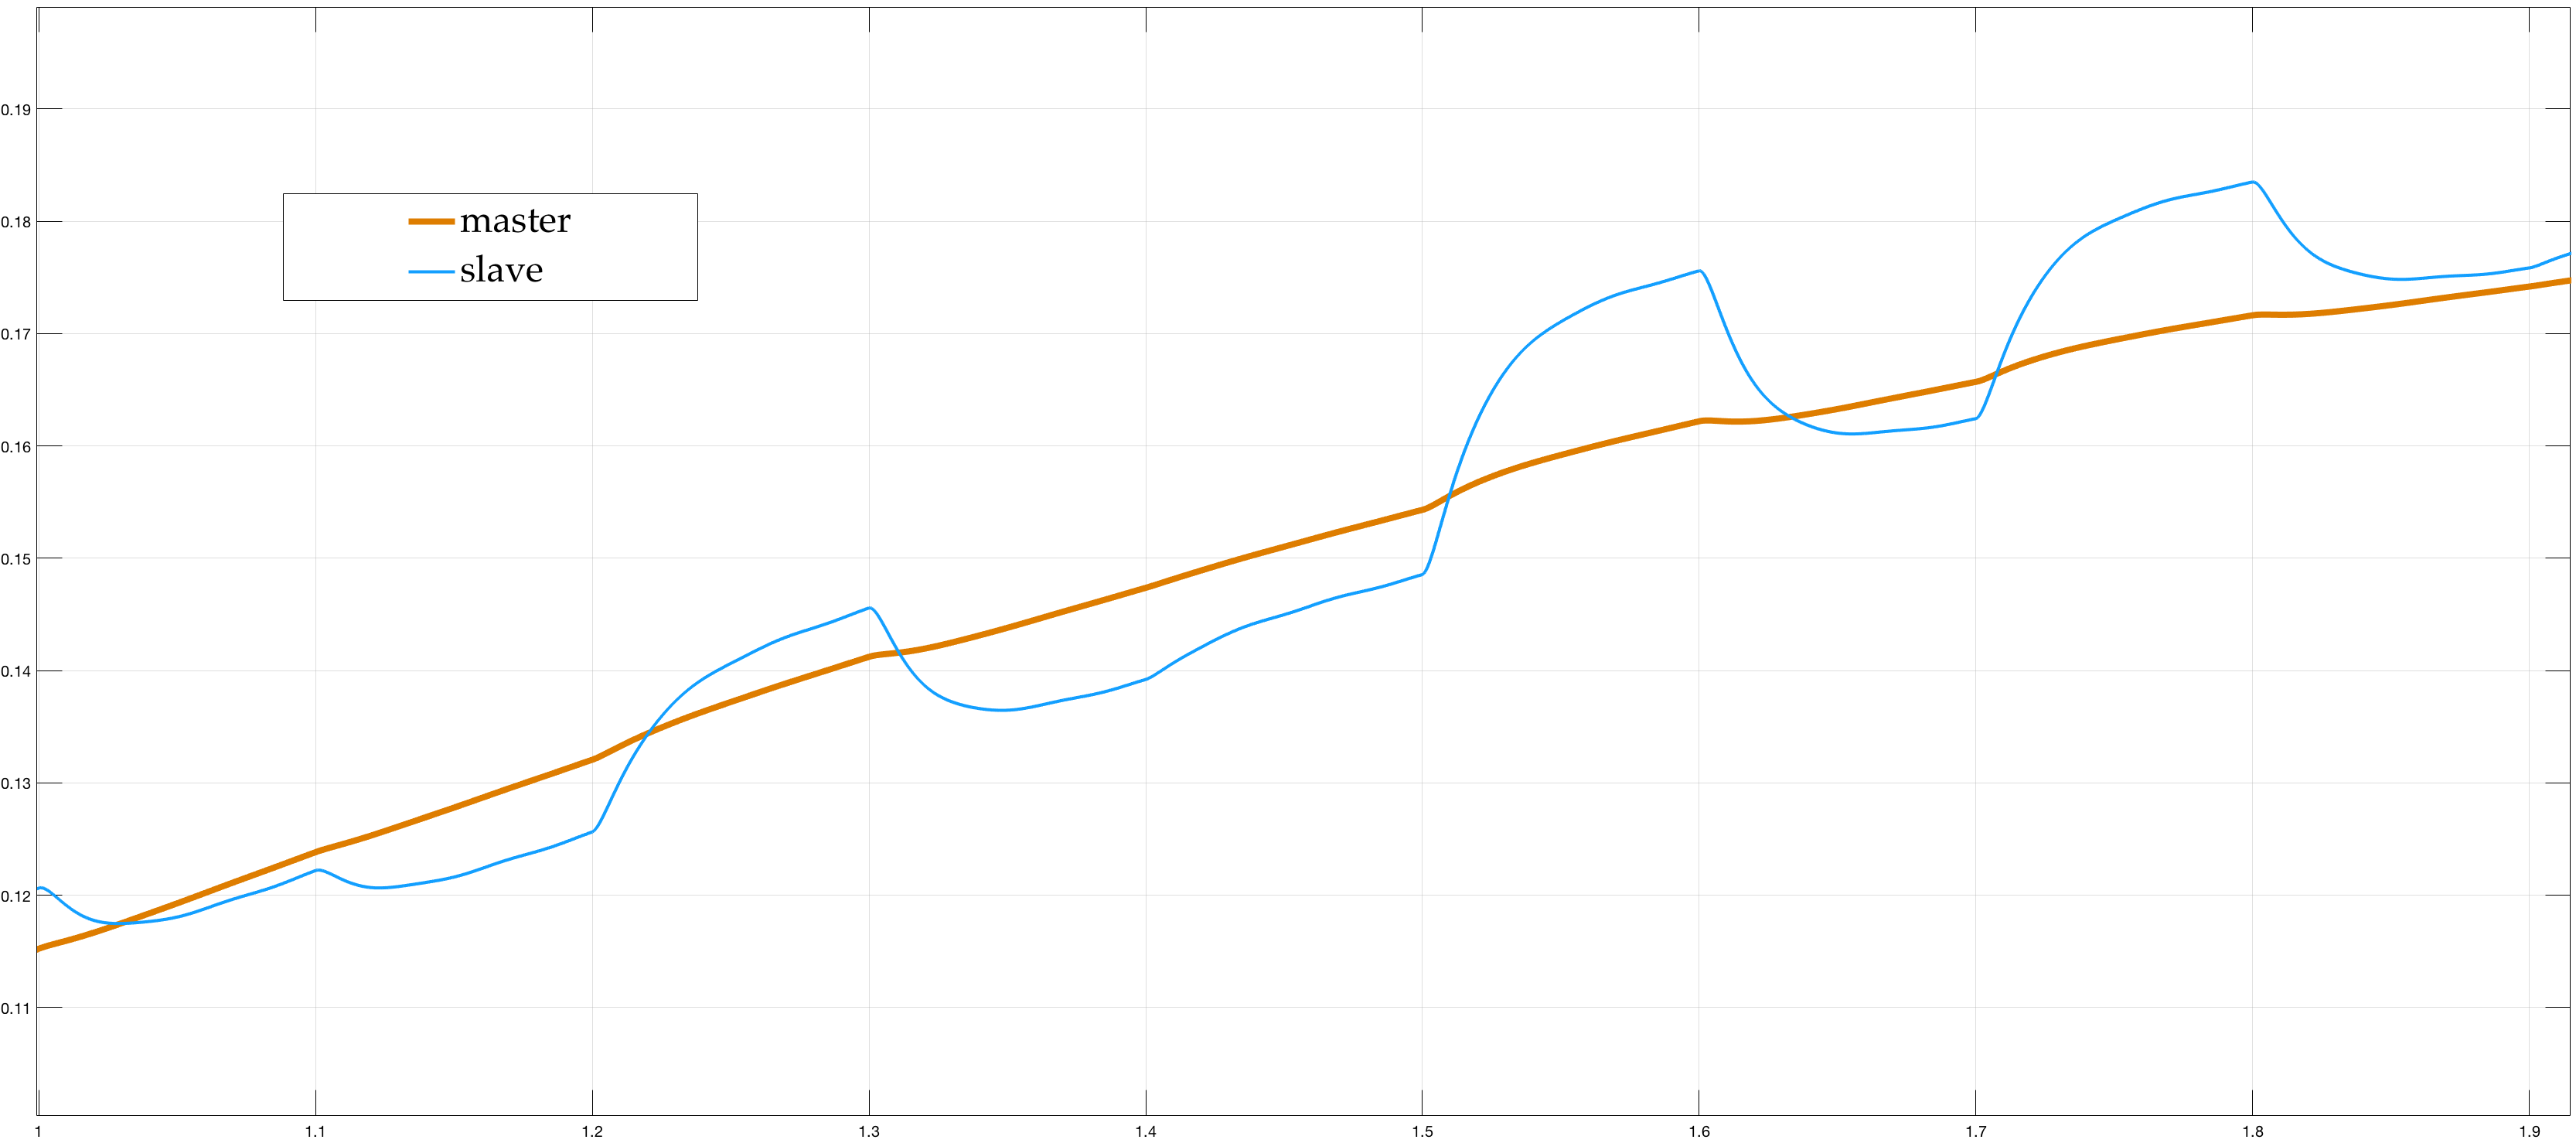
\includegraphics[width=\textwidth, height=0.48\textwidth]{Images/freeSet20Part20Htznoise}
		\caption{Detail describing the highlighted area in fig.\ref{fig:freeSetTot20HR}}
		\label{fig:freeSetPar20HR}
	\end{subfigure}	
  \caption{ Virtual compliance simulation under \textbf{low} frequency disturbances.}
\end{figure}

\newpage
\subsubsection{Environment contact }

In this section the proposed simulations hold the same reference trajectory for
master than the simulations in free motion.
\newline
But, in addiction, after that the slave would trespass a certain angle value
there would be a contact with the environment, this wouldn't allow a perfect
tracking by the slave.
\newline
The comparison between \textsl{ virtual compliance} and \textsl{rigid coupling}
in presence of an external force can be deduced by the
differences in \textbf{magnitude} of the arrows drawn in the figures below.

\begin{figure}[h]
	\begin{subfigure}[h!]{1\linewidth}
		\centering
		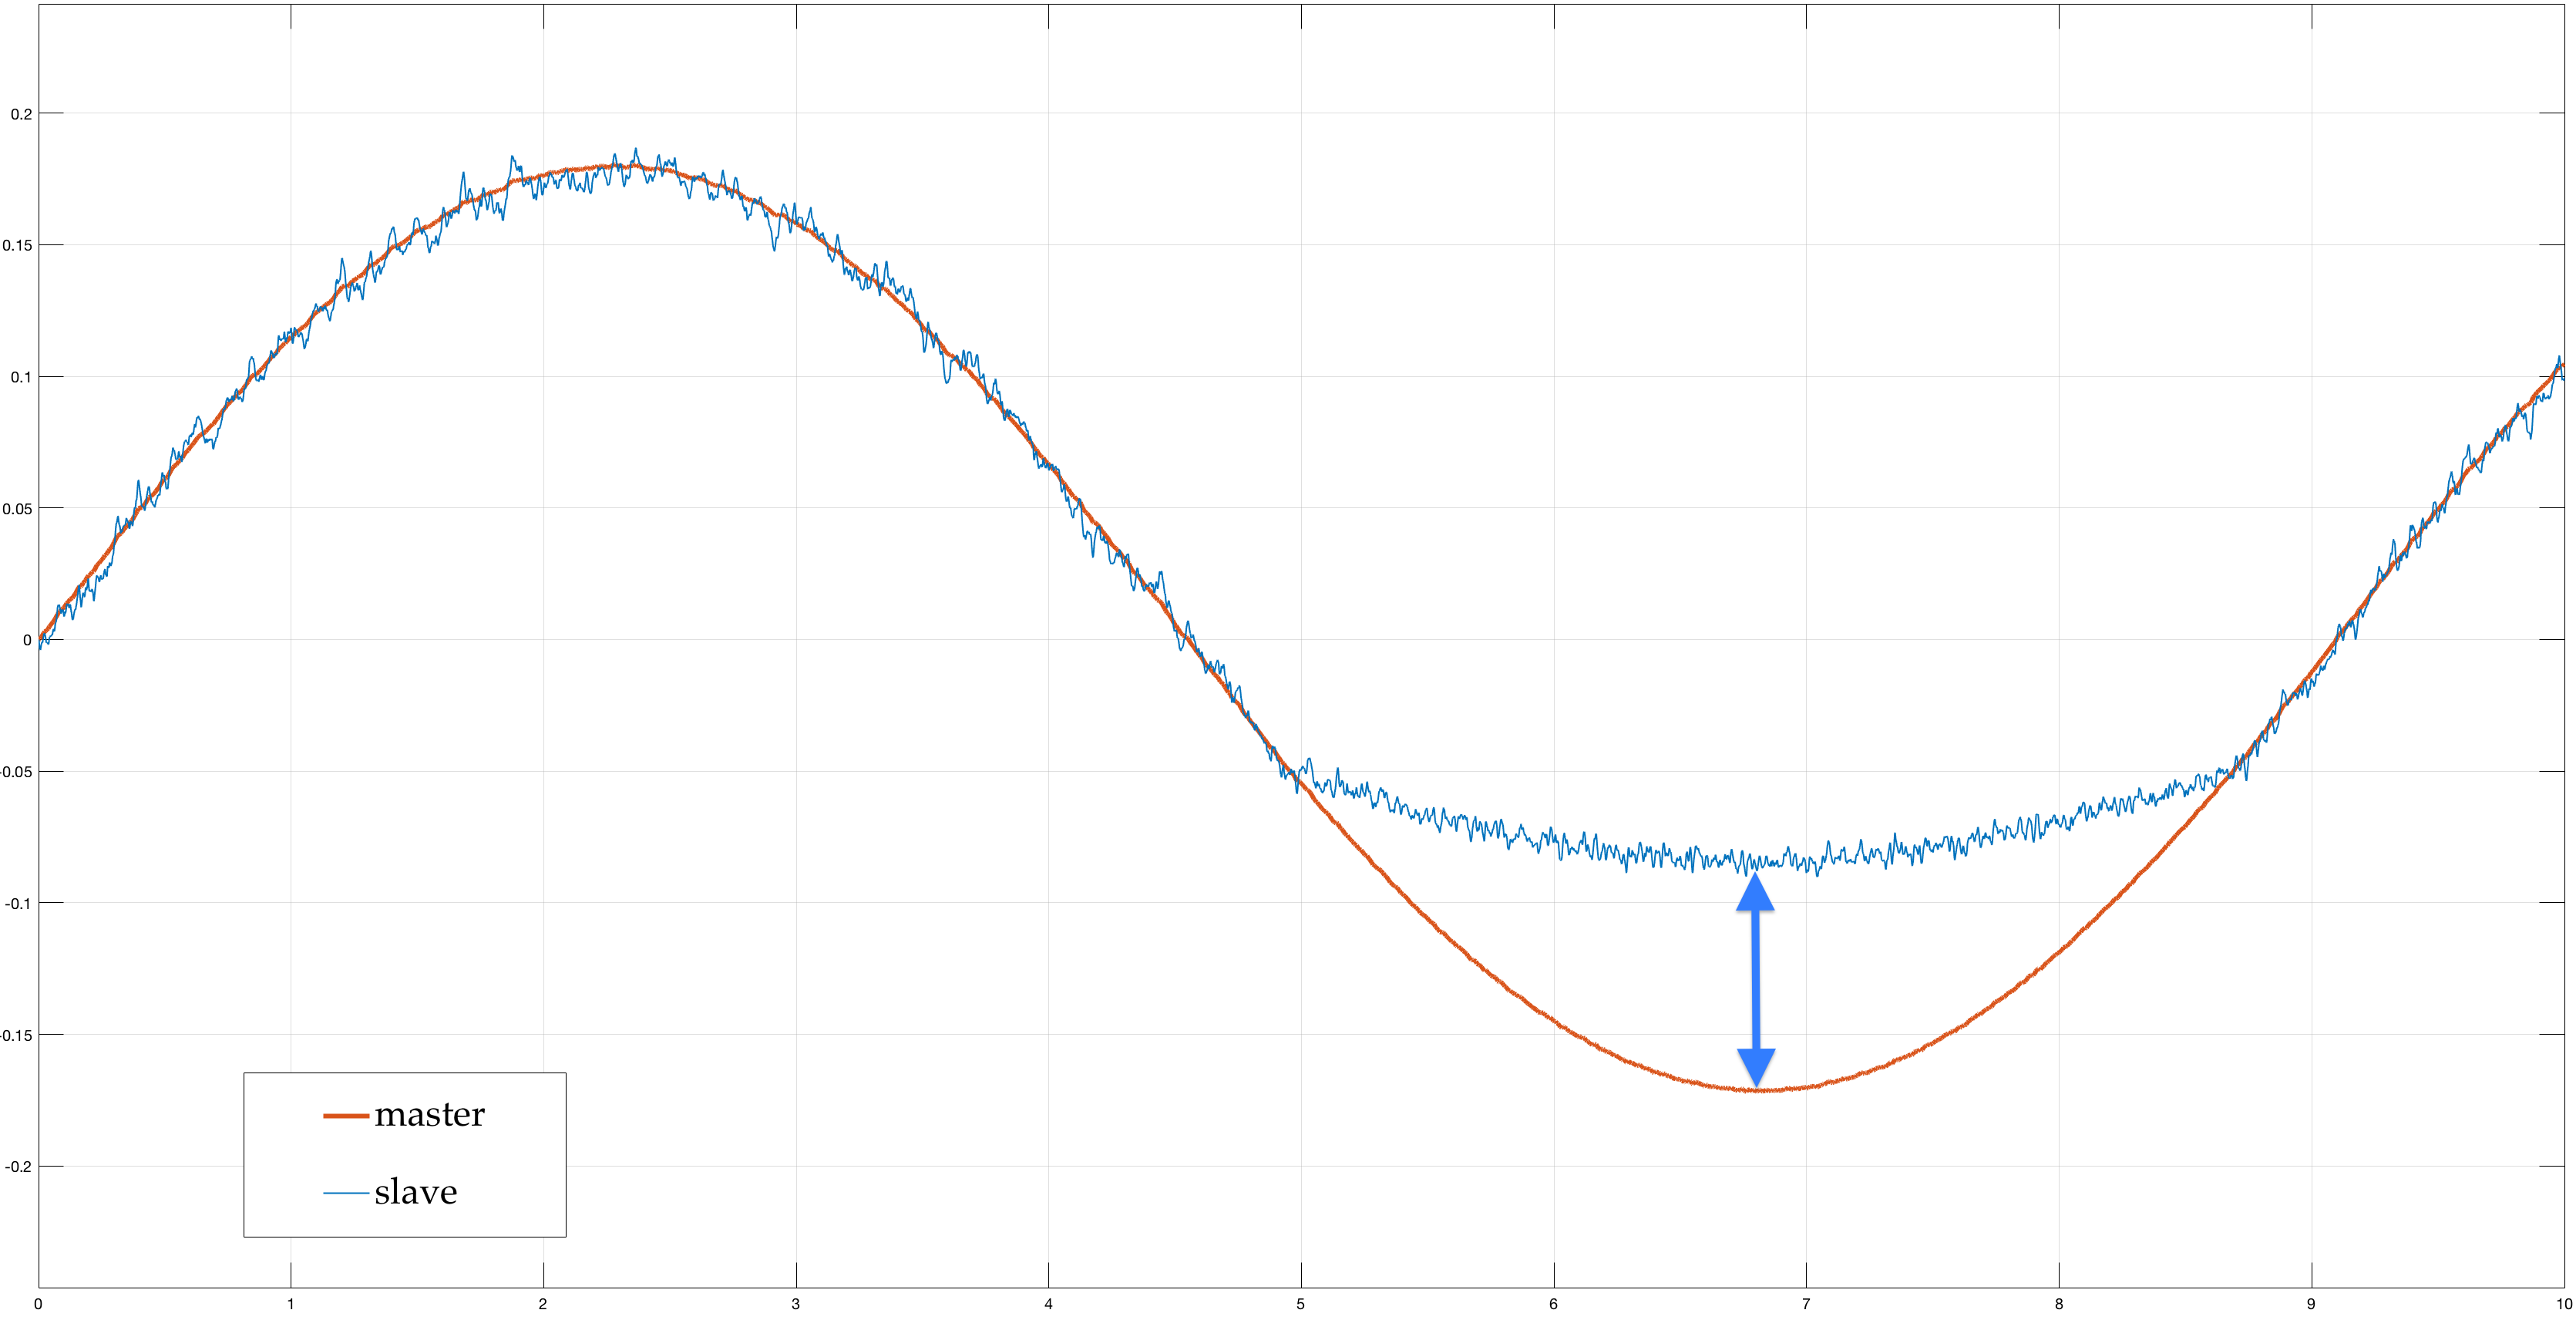
\includegraphics[width=\textwidth, height=0.45\textwidth]{Images/setPointContactReacPosArrow}
		\caption{ Angular position assumed during trajectory tracking.}
		\label{fig:ContactSetPos}
	\end{subfigure}	
  \newline
	\begin{subfigure}[h!]{1\linewidth}
		\centering
		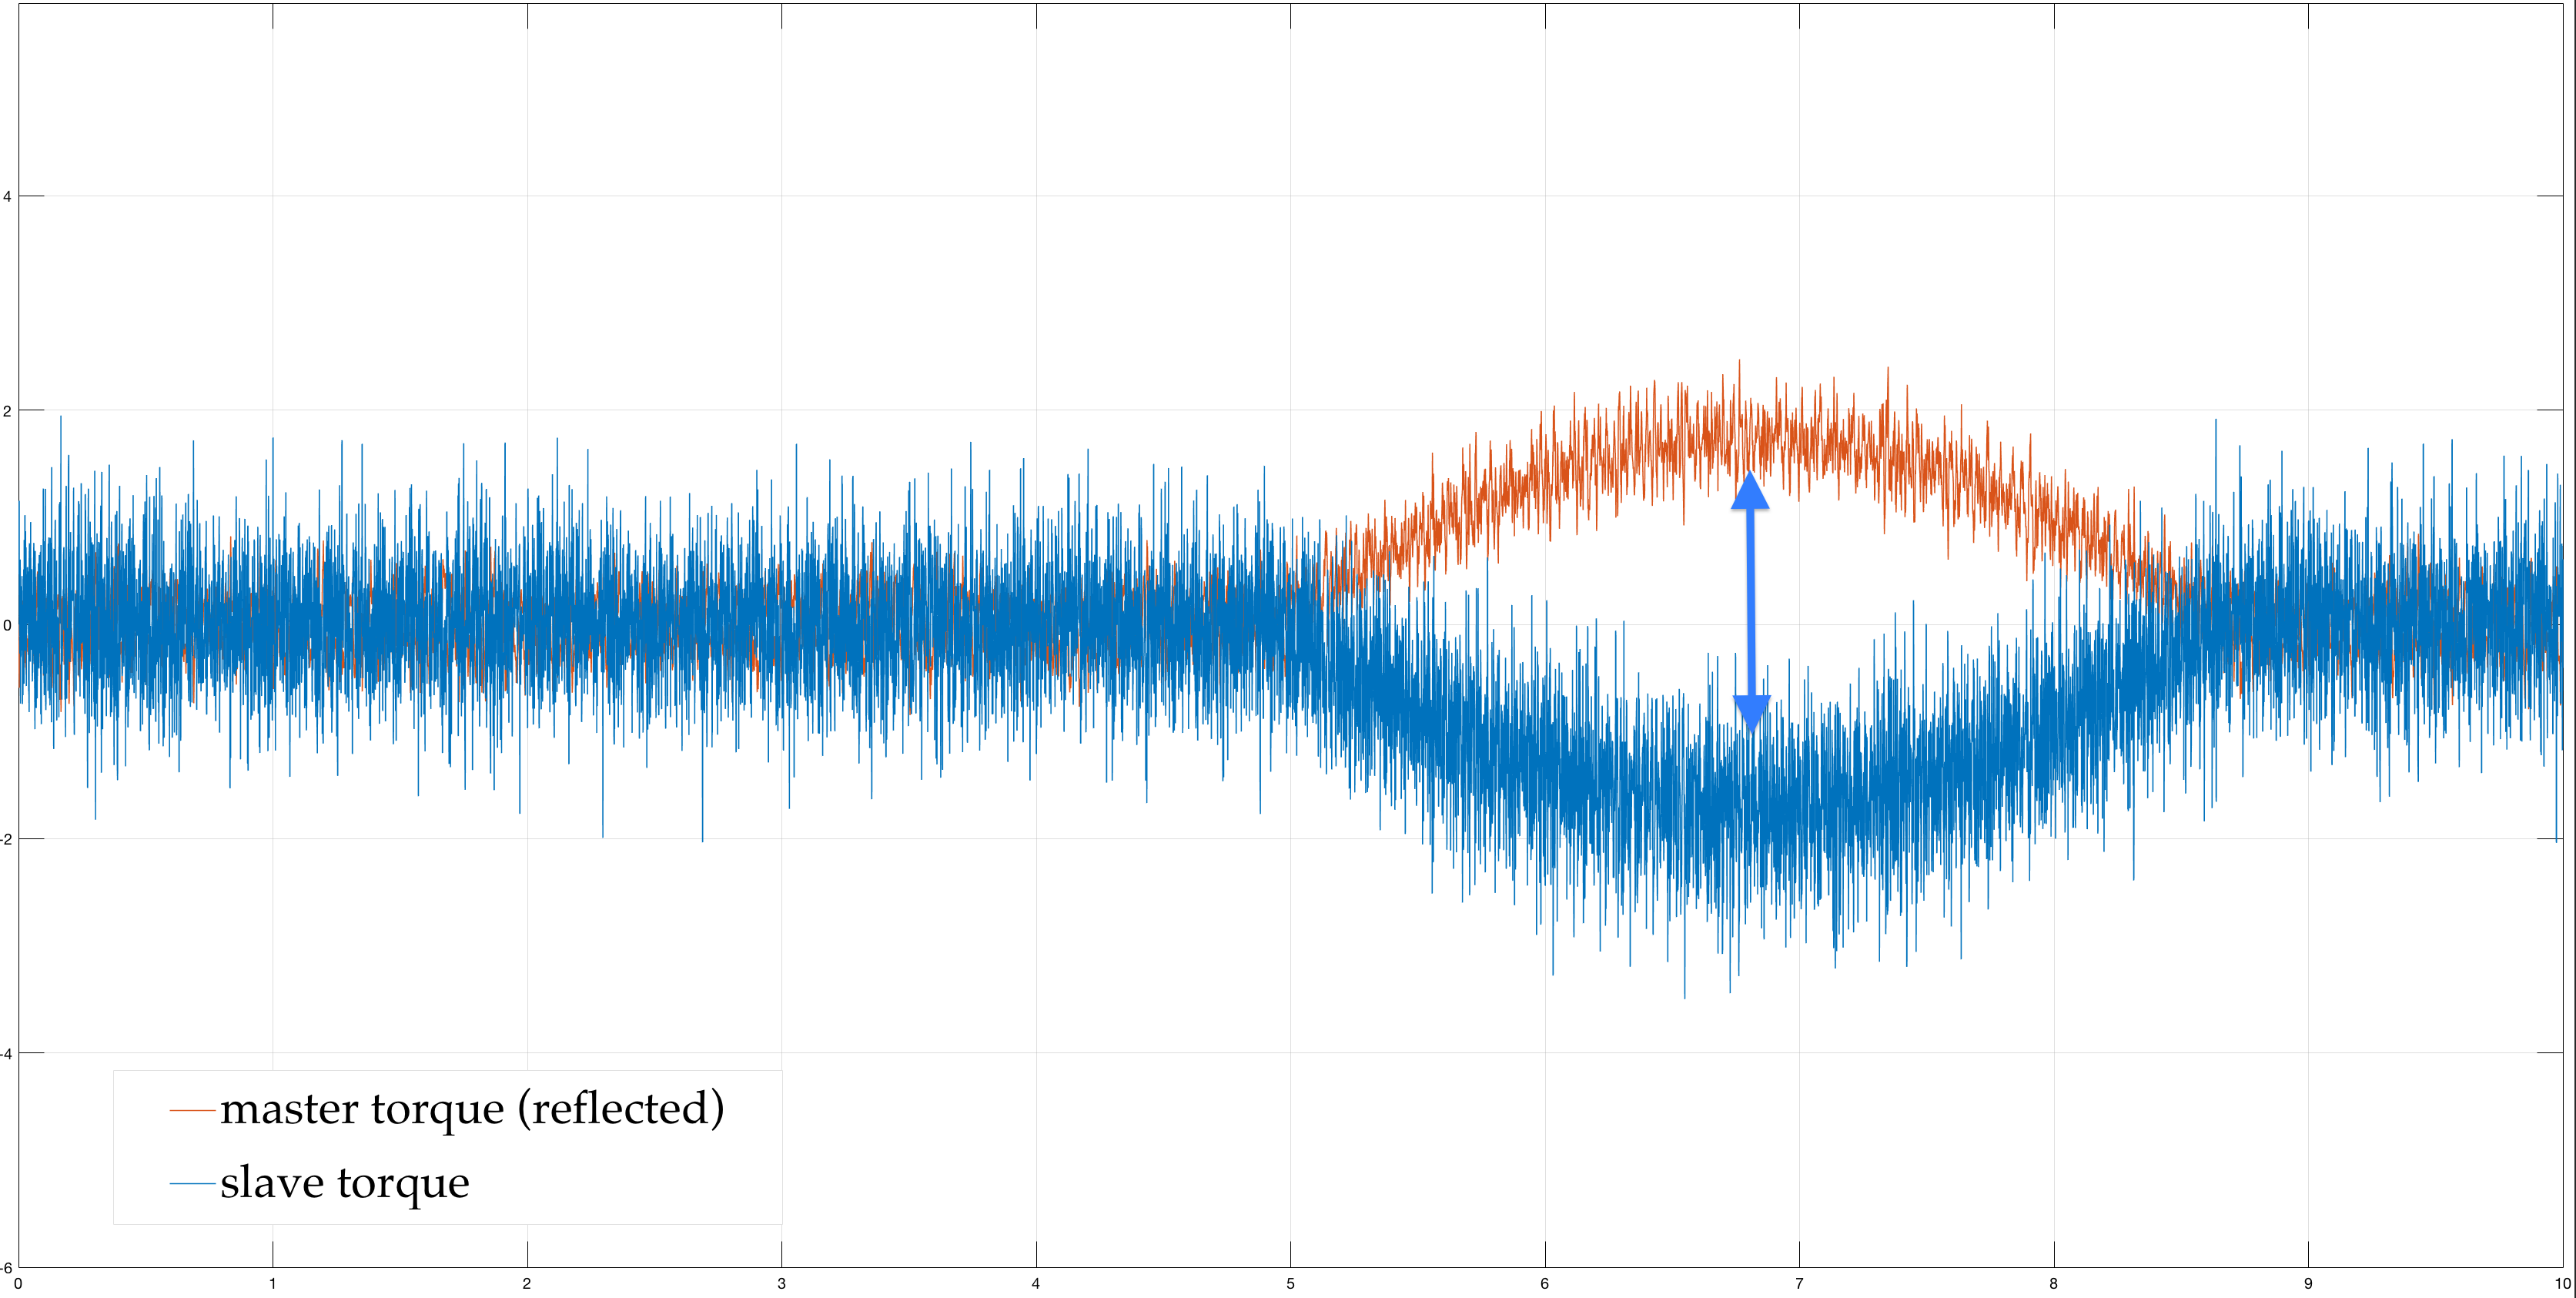
\includegraphics[width=\textwidth, height=0.45\textwidth]{Images/setPointContactReacTorArrow}
		\caption{ Torques exerted over time}
		\label{fig:ContactSetTor}
	\end{subfigure}	
 \caption{ Virtual compliance simulation in \textsl{contact} with
    the environment}
\end{figure}

Concerning the angular position of slave with the respect of master the
fig.\ref{fig:ContactSetPos} portraits a worse performance in trajectory error
when in contact behaving in \textsl{virtual compliance} than behaving in
\textsl{rigid coupling} (fig.\ref{fig:ContactRigPos}).
\newline
Instead, from the point of view of the torque exerted, the first approach
(fig.\ref{fig:ContactSetTor}) performs more efficiently than \textsl{rigid
  coupling} (fig.\ref{fig:ContactRigTor}).

  
\begin{figure}[h]
	\begin{subfigure}[h!]{1\linewidth}
		\centering
		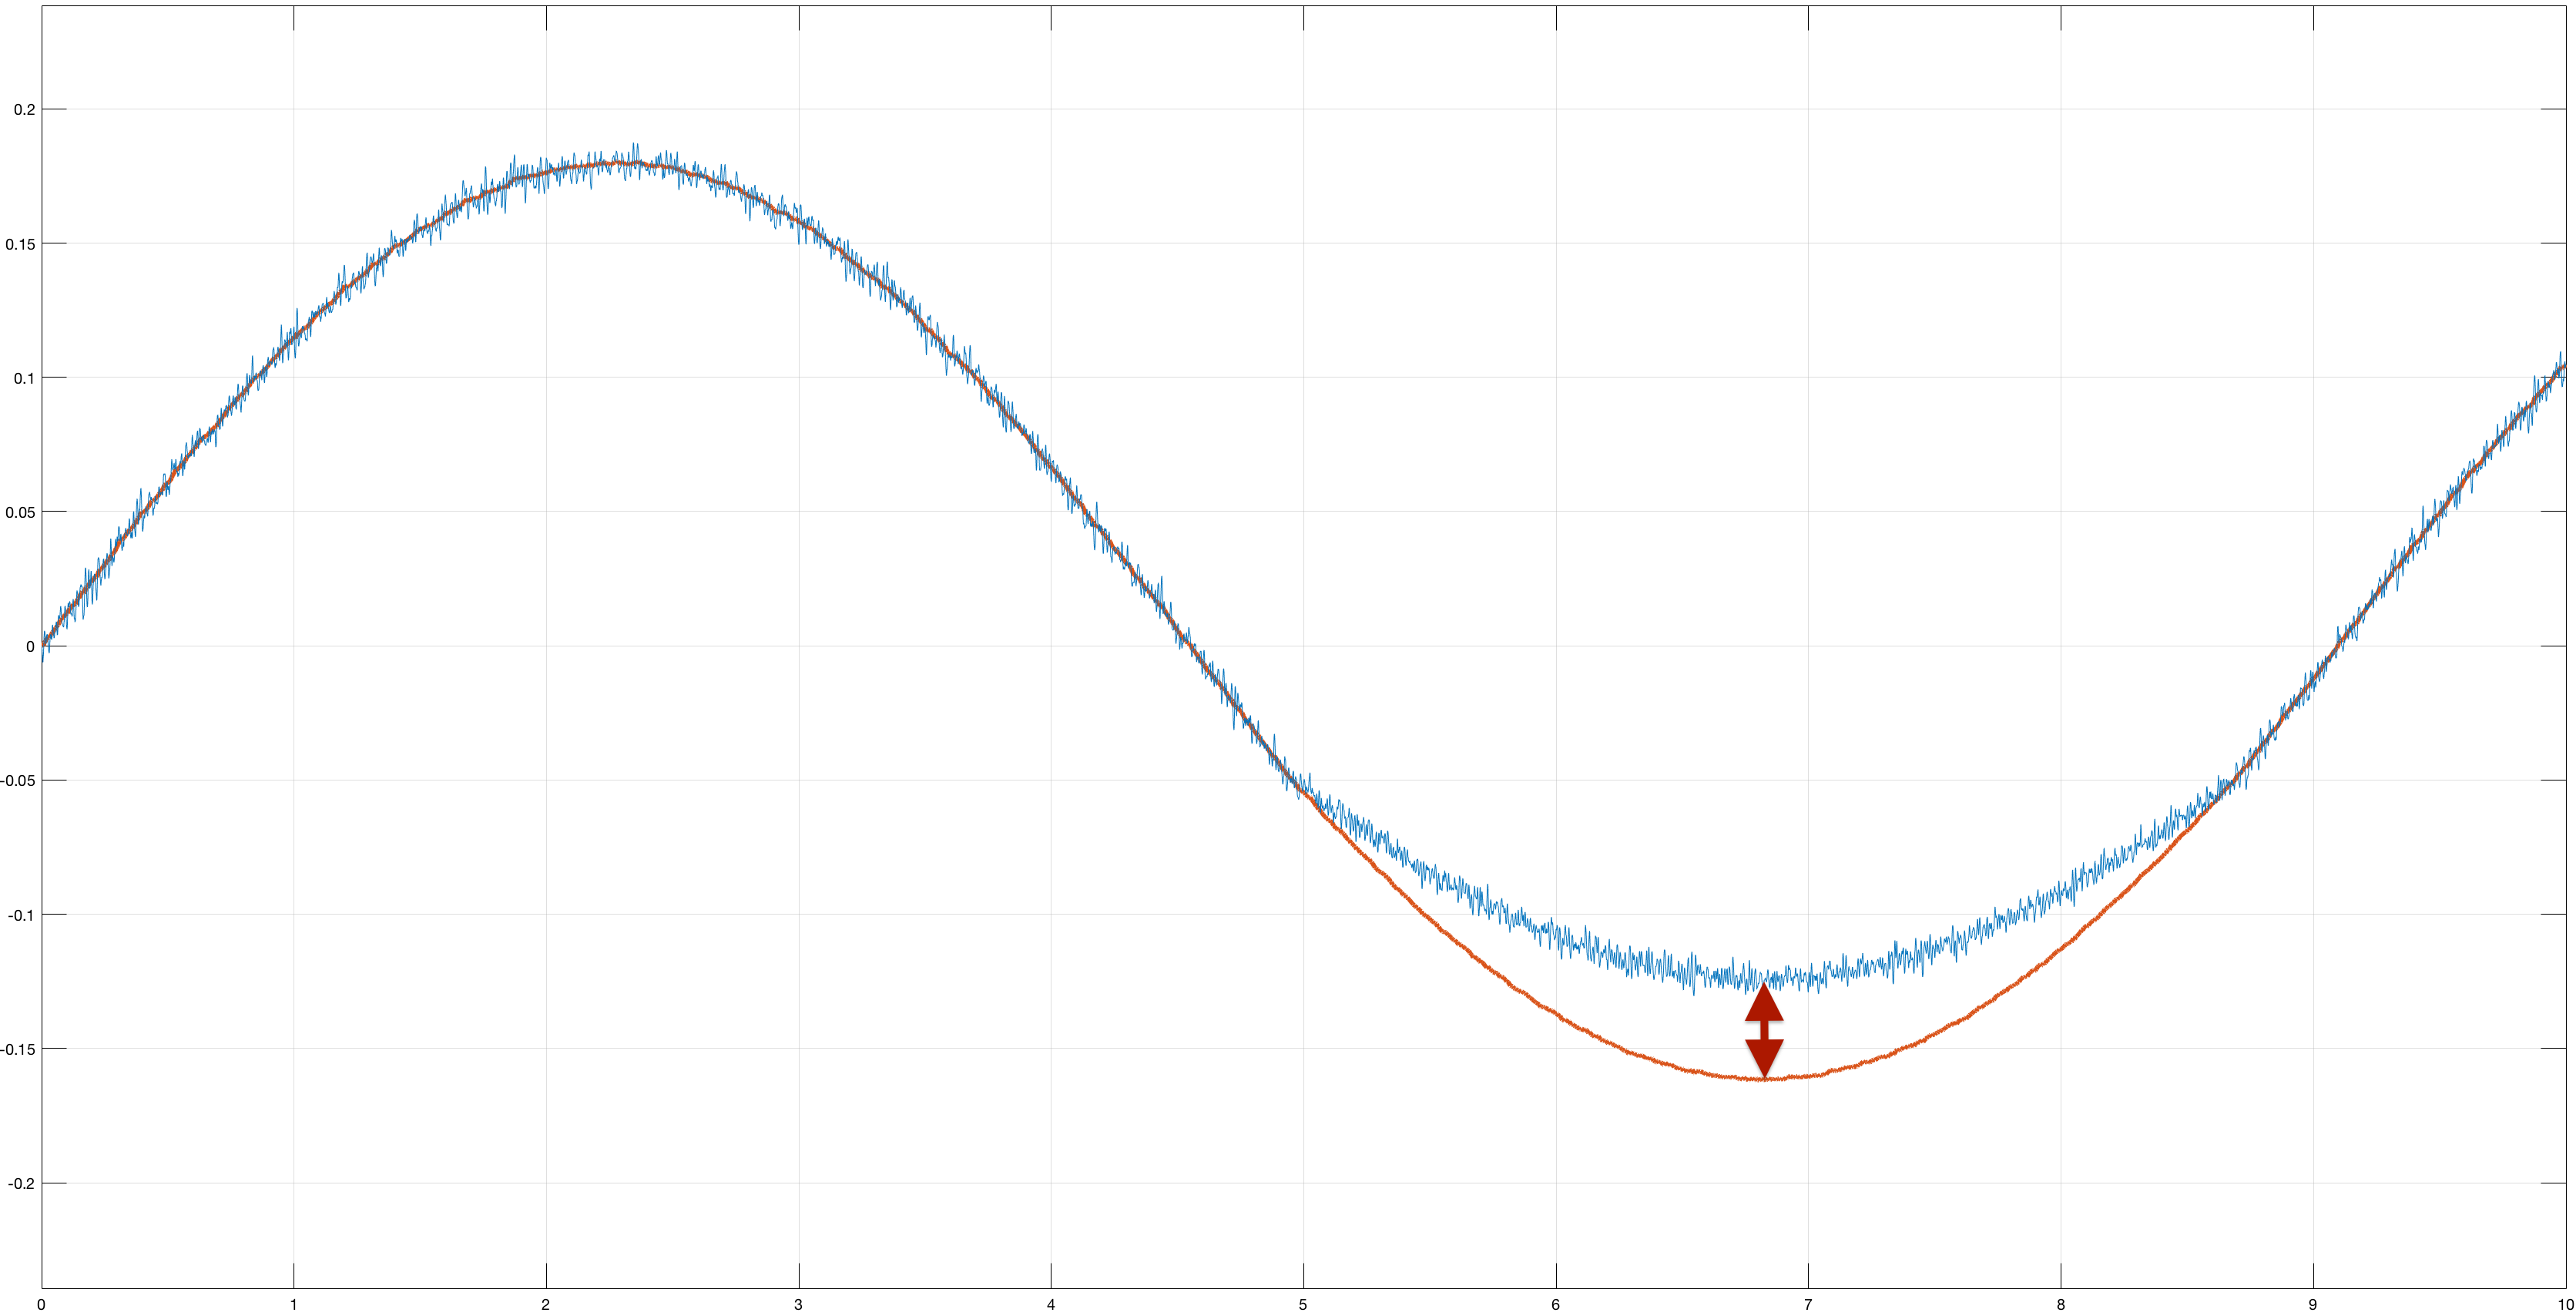
\includegraphics[width=\textwidth, height=0.45\textwidth]{Images/rigidContactReacPosArrow}
		\caption{ Angular position assumed during trajectory tracking.}
		\label{fig:ContactRigPos}
	\end{subfigure}	
  \newline
	\begin{subfigure}[h!]{1\linewidth}
		\centering
		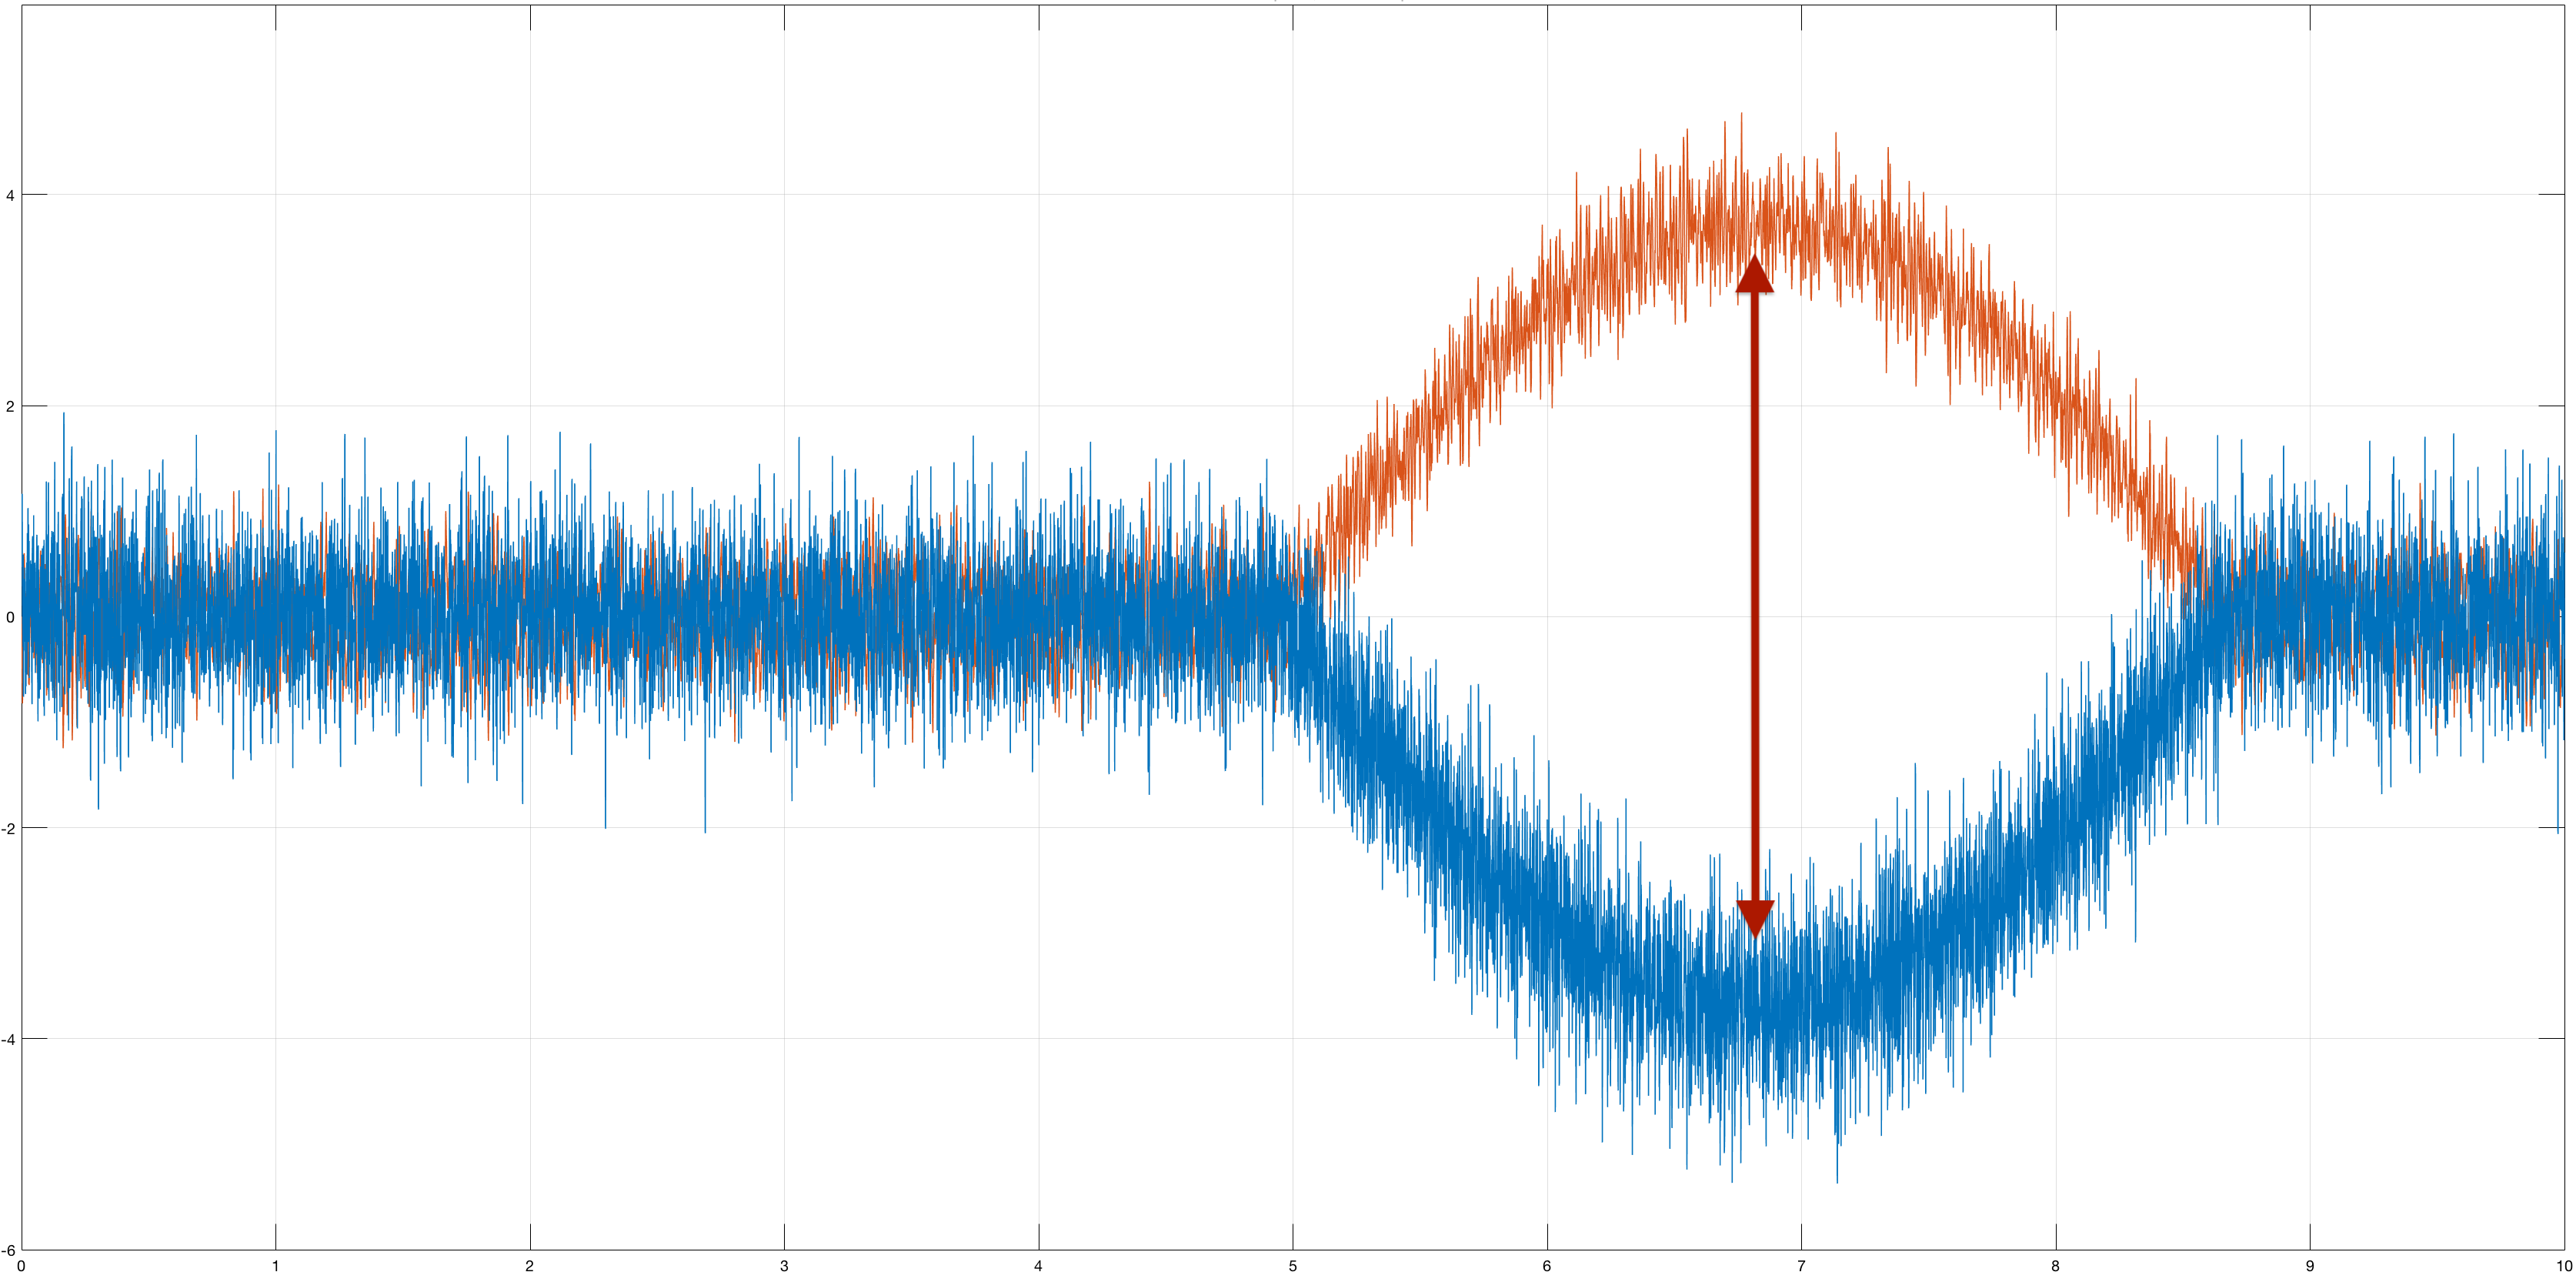
\includegraphics[width=\textwidth, height=0.45\textwidth]{Images/rigidContactReacTorArrow}
		\caption{ Torques exerted over time}
		\label{fig:ContactRigTor}
	\end{subfigure}	
  \caption{ Rigid coupling simulation in \textsl{contact} with
    the environment}
\end{figure}

\newpage
\section{Conclusions}
Vibration suppression in the contest of bilateral teleoperation is an open
issue.
\newline
The proposed solution based on a virtual spring-damper system with additional
inertia and a couple of cut-off frequencies that should be decided according to
the system requirements.
\bigskip
\newline
To summarize, when the virtual stiffness has been fixed,  the other virtual
parameters could be calculated from the equations in order to induce the desired
cut-off frequencies.
\bigskip
\newline
The vibration suppression performance shows promising results, since the
proposed virtually stiff approach can distinguish between useful signal
frequencies (\textsl{low}) and noisy ones (\textsl{high}). 
\bigskip
\newline
Overall, the tracking error in free motion is almost null. And regarding the contact with the environment is
interesting to observe from the simulations a trade-off
between control effort and task error.
\bigskip
\newline
Finally, the proposed bilateral control could be efficiently applied to tasks
that contemplate handling \textsl{soft} materials.



